\chapter{Simulation}
\label{chaptr:simulation}
 
%  There are several reasons why a simulation was used as a helpful tool alongside the real test-drives~\cite{wallentowitz1997vertikal}.
 
%%%%%%%%%%%%%%%%%%%%%%%%%%%%%%%%%%%%%%%%%%%%%%%%%%%%%%%%%%%%%%%%%%%%%%%%%%%%%%%%%%%%%%%%%%%%%%%%%%%
 \section{Road model}
 \label{sec:roadmodel}
 
 In general, the unevenness density of a road real profile decreases with an increase in spatial frequency.
%
The \ac{SPD} of a road profile is defined in \cite{_iso_2016} as 
\begin{align}\label{eq:psdiri}
G_d(\Omega) =
  \begin{cases}
    G_d(\Omega_0) \cdot \left(\dfrac{\Omega}{\Omega_0} \right)^{-n_1}  & \quad \text{if } \Omega \leq \frac{1}{2 \pi}\\
    G_d(\Omega_0) \cdot \left(\dfrac{\Omega}{\Omega_0} \right)^{-n_2}  & \quad \text{if } \Omega > \frac{1}{2 \pi}\\
  \end{cases},
\end{align}

where $\Omega = \frac{2\pi}{L}$ is the angular spatial frequency and $L$ the road length. Usually, $n_1=2$, $n_2=1.5$, $\Omega_0=1$ and the degree of roughness $G_d(\Omega_0)$ can be obtained from \cite{_iso_2016} for different road classes. It ranges from 0 (very smooth) to 8192 (very bad condition).
%
The unit of $G_d(\Omega_0)$ is $10^{-6}m^3$ and the unit of $\Omega_0$ is $rad/m$.
%
A random periodic road profile that fits the \ac{SPD} described in \eqref{eq:psdiri} can be generated with a Fourier series, the sum of individual sine waves, with~\cite{cebon_handbook_1999-1, agostinacchio_vibrations_2014}.

\begin{equation}
r(x)= \sum_{i=0}^{N}{\hat{p}_i \cdot \sin(2\pi \cdot i \cdot x+ \epsilon_i)}, \label{eq:RoadProf} 
\end{equation}

which lead us to
\begin{equation}
r(x)= \sum_{i=0}^{N}{\sqrt{2 \cdot \Delta\Omega \cdot G_d(i\cdot\Delta\Omega)} \cdot \sin(2\pi \cdot i \cdot x \cdot \Delta\Omega + \epsilon_i)}. \label{eq:genRoadProf}
\end{equation}
%
$\Delta\Omega$ is the frequency band and $\epsilon_i$ as a random phase angle uniformly distributed between $0$ and $2\pi$.

Furthermore, we have added road features to our road profile, including potholes, manhole cover, railway crossing and cobbled road.
%
It is described through suitable functions with varying parameters in a specific range, e.g. the depth or height $h$ and the length $l$ of such road features.
%
Hereby, an obstacle described by a non-continuously differentiable function can cause numerical issues in the time step integration process of the simulation itself~\cite{frey2012development}.
%
Thus the transition part of the road features should be smooth. The function and the profile of the road features are shown as below.

\begin{align}
    f_\text{pothole}(x)&=\frac{h}{2}\cdot (cos(\frac{2\pi}{l} \cdot x)-1) \quad (0\leq x \leq l),
    \\
f_\text{manhole\_cover}(x)&=
\begin{cases}
    \frac{h}{2}\cdot (1-cos(\frac{12 \pi}{l}\cdot x))  & (0\leq x \leq \frac{l}{12}) \\
    1              & (\frac{l}{12} \leq x \leq \frac{11l}{12}) \\
    \frac{h}{2}\cdot (1+cos(\frac{12 \pi}{l}\cdot (x-\frac{11l}{12})))  & (\frac{11l}{12} \leq x \leq l)
\end{cases},
\\
    f_\text{cobble\_left}(x) &=\frac{h}{2}\cdot (1-cos(\frac{2\pi}{l} \cdot x)) \quad (0\leq x \leq l), \\
    f_\text{cobble\_right}(x)&=\frac{h}{2}\cdot (1+cos(\frac{2\pi}{l} \cdot x)) \quad (0\leq x \leq l),
\\
f_\text{railway\_crossing}(x) &=
\begin{cases}
    \frac{h}{2}\cdot (cos(\frac{80 \pi}{l}\cdot x)-1) & (0\leq x \leq \frac{l}{80}) \\
    0             & (\frac{l}{80} \leq x \leq \frac{l}{16}) \\
    \frac{h}{2}\cdot (cos(\frac{80 \pi}{l}\cdot (x-\frac{5l}{80}))+1) & (\frac{5l}{80} \leq x \leq \frac{6l}{80}) \\
    0             & (\frac{6l}{80} \leq x \leq \frac{74l}{80}) \\
    \frac{h}{2}\cdot (cos(\frac{80 \pi}{l}\cdot (x-\frac{74l}{80}))-1) & (\frac{74l}{80} \leq x \leq \frac{75l}{80}) \\
    0             & (\frac{75l}{80} \leq x \leq \frac{79l}{80}) \\
    \frac{h}{2}\cdot (cos(\frac{80 \pi}{l}\cdot (x-\frac{79l}{80}))+1) & (\frac{79l}{80} \leq x \leq l)
\end{cases}.
\end{align}


\begin{figure}
 \centering
 \begin{tikzpicture}
 \begin{groupplot}[mygroupplot,
 group style={group name=my plots,group size= 2 by 2, horizontal sep=\myGroupSep, 
 vertical sep=\myGroupVertSep},
 ]
 		
 	\nextgroupplot[
	xlabel=Distance ($m$),
	ylabel=Height ($m$),
	%ymin=-0.01,   
	%ymax=0.03,
	%ymin=100,   
	%ymax=120,
%	legend columns=1,
%	legend entries={with anti-roll bar, without anto roll bar},
%	legend style={at={\myLegendPosition},anchor=south,name=leg},
    cycle list name=mycyclelist,
    ]
    \newcommand{\point}{5};
    \addplot+[no marks, each nth point=\point] table[x=r,y=h] {data/pothole.txt};
 
 
  	\nextgroupplot[
	xlabel=Distance ($m$),
	ylabel=Height ($m$),
	%ymin=-0.01,   
	%ymax=0.03,
	%ymin=100,   
	%ymax=120,
	%legend columns=1,
	%legend entries={,$sin(x)+0.5$},
	%legend style={at={\myLegendPosition},anchor=south,name=leg},
    cycle list name=mycyclelist,
    ]
    \newcommand{\point}{5};
    \addplot+[no marks, each nth point=\point] table[x=r,y=h] {data/manhole.txt};
    
    \nextgroupplot[
	xlabel=Distance ($m$),
	ylabel=Height ($m$),
	%ymin=-0.01,   
	%ymax=0.03,
	%ymin=100,   
	%ymax=120,
	%legend columns=1,
	%legend entries={,$sin(x)+0.5$},
	%legend style={at={\myLegendPosition},anchor=south,name=leg},
    cycle list name=mycyclelist,
    ]
    \newcommand{\point}{5};
    \addplot+[no marks, each nth point=\point] table[x=r,y=h] {data/cobbled.txt};
    
    \nextgroupplot[
	xlabel=Distance ($m$),
	ylabel=Height ($m$),
	%ymin=-0.01,   
	%ymax=0.03,
	%ymin=100,   
	%ymax=120,
	%legend columns=1,
	%legend entries={,$sin(x)+0.5$},
	%legend style={at={\myLegendPosition},anchor=south,name=leg},
    cycle list name=mycyclelist,
    ]
    \newcommand{\point}{5};
    \addplot+[no marks, each nth point=\point] table[x=r,y=h] {data/crack.txt};
 
 \end{groupplot}

\node[below = \myLabelSep of my plots c1r1.south] {pothole};
\node[below = \myLabelSep of my plots c2r1.south] {manhole cover};
\node[below = \myLabelSep of my plots c1r2.south] {cobbled road};
\node[below = \myLabelSep of my plots c2r2.south] {railway crossing};

 \end{tikzpicture}
 \label{fig:road_events}
 \caption{Generated road profile for simulation of car models described in Sections~\ref{sec:antirollbar} to \ref{sec:positionofoutput}. Left and right profiles are different to investigate the influence of the anti-roll bar.}
 \end{figure}
 

% One concern that is unique to the simulation of tire models as they traverse a rectangular cleat is the instantaneous change in vertical velocity or at least a change that is more rapid than the actual physical system can cause 

Fig.~\ref{fig:road_profile_1} shows the generated road profile, which is used to show the influences of various extensions of the full car model in Sections~\ref{sec:antirollbar} to \ref{sec:positionofoutput}.

 \begin{figure}
 \centering
 \begin{tikzpicture}
 \begin{groupplot}[mygroupplot,
 group style={group name=my plots,group size= 2 by 1, horizontal sep=\myGroupSep, 
 vertical sep=\myGroupVertSep},
 ]
 		
 	\nextgroupplot[
	xlabel=Distance ($m$),
	ylabel=Height ($m$),
	ymin=-0.01,   
	ymax=0.03,
	%ymin=100,   
	%ymax=120,
%	legend columns=1,
%	legend entries={with anti-roll bar, without anto roll bar},
%	legend style={at={\myLegendPosition},anchor=south,name=leg},
    cycle list name=mycyclelist,
    ]
    \newcommand{\point}{5};
    \addplot+[no marks, each nth point=\point] table[x=r,y=h1] {data/road_profile1.txt};
 
 
  	\nextgroupplot[
	xlabel=Distance ($m$),
	ylabel=Height ($m$),
	ymin=-0.01,   
	ymax=0.03,
	%ymin=100,   
	%ymax=120,
	%legend columns=1,
	%legend entries={,$sin(x)+0.5$},
	%legend style={at={\myLegendPosition},anchor=south,name=leg},
    cycle list name=mycyclelist,
    ]
    \newcommand{\point}{5};
    \addplot+[no marks, each nth point=\point] table[x=r,y=h2] {data/road_profile1.txt};
 
 \end{groupplot}

\node[below = \myLabelSep of my plots c1r1.south] {left: $G_d(\Omega_0)=8$ and oscillations};
\node[below = \myLabelSep of my plots c2r1.south] {right: $G_d(\Omega_0)=8$};

 \end{tikzpicture}
 \label{fig:road_profile_1}
 \caption{Generated road profile for simulation of car models described in Sections~\ref{sec:antirollbar} to \ref{sec:positionofoutput}. Left and right profiles are different to investigate the influence of the anti-roll bar.}
 \end{figure}
 

%%%%%%%%%%%%%%%%%%%%%%%%%%%%%%%%%%%%%%%%%%%%%%%%%%%%%%%%%%%%%%%%%%%%%%%%%%%%%%%%%%%%%%%%%%%%%%%%%%%
\section{Basic full car model}
\label{sec:full car model}
 
The basic full car model consists of springs, dampers, masses and incorporates pitch and roll motion, giving a total of seven \ac{DOF}.
%
Consequently it can present more details of the behavior of the vehicle traversing different road situation.
%
The mass of axle is distributed to the vehicle body and the mass of the wheel and tire is modeled as a mass point.
%
To simplify the calculation, the roll center and pitch center of the vehicle are assumed to coincide in the gravity center.
%
Besides, we set 1, 2 as the front-right and front-left wheel and 3, 4 as the rear-right and rear-left wheel.

Since the damper of the tire is very small compared to the damper of the suspension, it can be neglected.
%
A damper limits the resonant response of the vehicle vibration due to the suspension springs is non-linear.
%
However, the transmission behavior of the axis has improved its linearity until the wheel frequency due to the interaction between the ripple of the roadway excitation and the transfer behavior of the axis. 
%
This advocates the use of linear transfer functions to characterize the vibration comfort~\cite{iliev2014systemansatz}.
%
Thus the passive suspension system between the sprung mass and unsprung masses was modeled as a linear spring and viscous damper at each corner.

The front suspension of the test vehicle BMW 116d is the MacPherson suspension and the rear suspension of it is multi-link suspension.
%
It is well known that the strut of these suspension is not directly connected to the center of the tire.
%
Moreover, the strut of the MacPherson suspension especially has an angle relative to the vertical line of the tire.
%
The method to describe the suspension can be found in~\cite{jazar2008vehicle}, which is shown in Fig.~\ref{fig:susp}.

 \begin{figure}
 \centering
 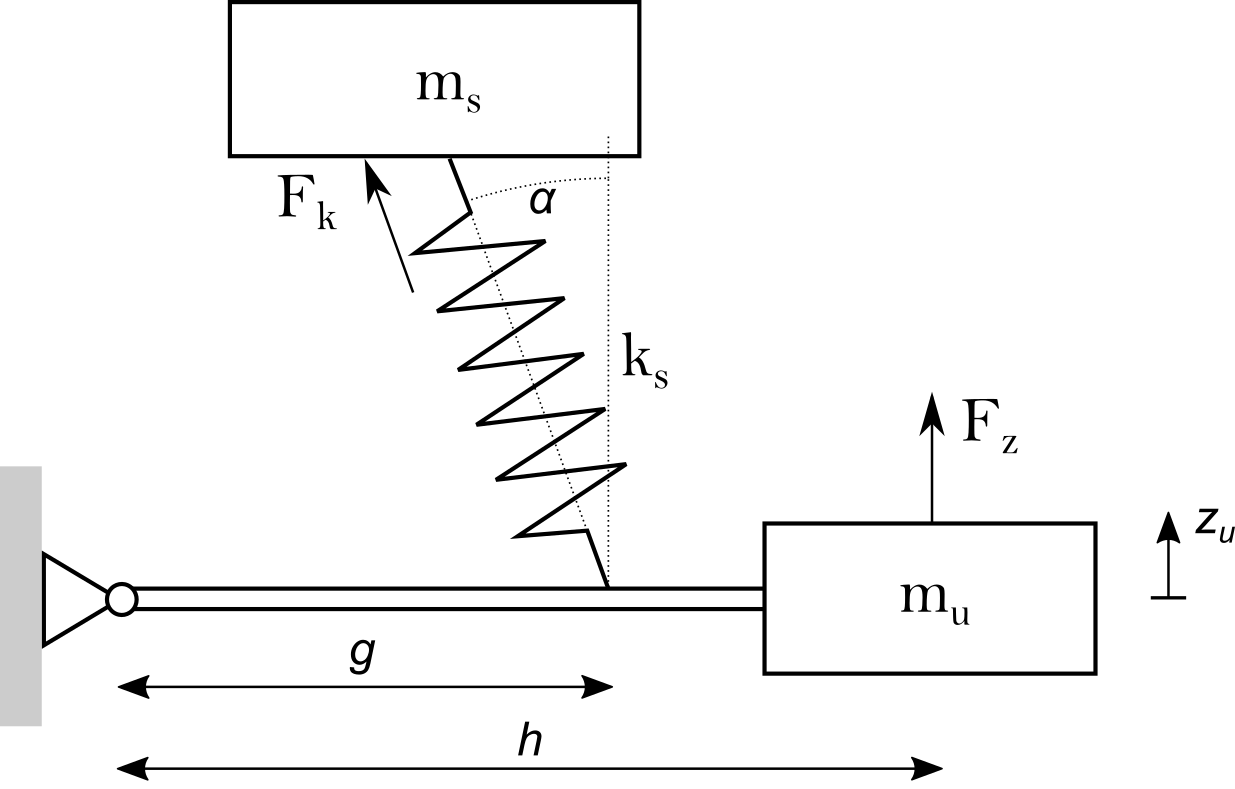
\includegraphics[width=0.5\textwidth]{bilder/suspension.png}
 \caption{The strut equivalent schematic}
 \label{fig:susp}
 \end{figure}

Regardless of the damper, the spring elongation $\delta_u$ is

\begin{equation}
    \delta_u = -\frac{g}{h} cos\alpha \cdot z_u
\end{equation}

According to the spring elongation, the spring force $F_k$ is

\begin{equation}
    F_k = -k_s\delta_u = k_s\frac{g}{h} cos\alpha \cdot z_u
\end{equation}

It is now possible to substitute the tilted spring elongation with an equivalent spring elongation $z_{eq}$ on the z-axis that needs the same force $F_z$, to elongate the same amount as the mass moves.
%

\begin{equation}
    z_{eq} = \frac{g}{h} cos\alpha \cdot z_u
\end{equation}

The vertical component of the force on the unsprung mass can be calculated by

\begin{equation}
    F_z = \frac{g}{h} cos\alpha \cdot F_k
\end{equation}

Thus the relationship can be describe by a equivalent coefficient $i$, the force on the sprung mass $F$ and on the unsprung mass $F_z$ are

\begin{align}
    F &= -cos\alpha \cdot (k_s(z_s - i\cdot z_u)+d_s(\dot{z_s}-i\cdot \dot{z_u})) \\
    F_z &= i\cdot (k_s(z_s - i\cdot z_u)+d_s(\dot{z_s}-i\cdot \dot{z_u}))
\end{align}

where

\begin{equation}
    i = \frac{g}{h} cos\alpha
\end{equation}

The equivalent coefficient $i$ is relative to the dimension of the structure of the suspension.
%
Due to the unavailable devices for the measurement of the length and angle of the strut, the coefficient is temporarily assumed as one.
%
Here i ignore the influence by the mechanic structure of the suspension.

With the above mentioned assumptions the \ac{FCM} is shown in Fig.~\ref{fig:fullcar},

\begin{figure}%
\footnotesize
\centering
\pgfdeclarelayer{bg}    % declare background layer
\pgfsetlayers{bg,main}
\begin{tikzpicture}
%\draw (-8.7,-2.7) rectangle (2,3.7);
\clip (-8.7,-2.7) rectangle (2,3.7);
		\def\lengthstreet{0.6cm};
		\def\spacerstreet{0cm};
		\def\tireheight{0.4cm};
		\def\tirewidth{0.8cm};
		\def\vectorlength{0.39cm};
		\def\labledistanceleft{0.0cm};
		\def\labledistanceright{0.15cm};
		\def\myyshift{-0.19cm}
		
		\def\a{-0.2cm};
		\def\b{-1.3cm};
		\def\c{-2.8cm};
		\def\d{0.21cm};
		\tikzstyle{line}=[];
     \tikzstyle{spring}=[line,decorate,decoration={zigzag,pre length=0.3cm,post length=0.3cm,segment length=6}]
		 
     \tikzstyle{strasse}=[line,decorate,decoration={snake,pre length=0cm,post length=0.0cm,segment length=30, amplitude = 0.1cm}]%, pattern = north east lines] 
     \tikzstyle{dampener}=[line,decoration={markings, mark connection node=dmp,mark=at position 0.5 with {
     \node (dmp) [line,inner sep=0pt,transform shape,rotate=-90,minimum width=15pt,minimum height=3pt,draw=none] {};
     \draw [line] ($(dmp.north east)+(2pt,0)$) -- (dmp.south east) -- (dmp.south west) -- ($(dmp.north west)+(2pt,0)$); \draw [line] ($(dmp.north)+(0,-5pt)$) -- ($(dmp.north)+(0,5pt)$);}}, decorate]
     \tikzstyle{ground}=[fill,pattern=north east lines,draw=none,minimum width=4cm,minimum height=0.3cm]

		\newcommand\centerofmassfc{%
    \tikz[radius=0.4em] {%
        \fill (0,0) -- ++(0.4em,0) arc [start angle=0,end angle=90] -- ++(0,-0.8em) arc [start angle=270, end angle=180];%
        \draw (0,0) circle;%
			}%
		}
     \begin{scope}
		
		
  \coordinate (A0) at (-7cm,0.5cm);% node at (A0){A0}; % central top point (To pick)
	\coordinate (A1) at ($(A0) + (0cm,\a)$);% node at (A1){A1}; % central top point (To pick)
	\coordinate (A3) at ($(A1) + (0cm,\c)$);
	
	
	\coordinate (B0) at (-2.5cm,1.7cm);% node at (B0){B0}; % right vanishing point (To pick)
	\coordinate (B1) at ($(B0) + (0cm,\a)$);% node at (B1){B1}; % right vanishing point (To pick)
	\coordinate (B3) at ($(B1) + (0cm,\c)$);
	
	
	\coordinate (C0) at (0cm,1.7cm);% node at (C0){C0}; % left vanishing point (To pick)
	\coordinate (C1) at ($(C0) + (0cm,\a)$);% node at (C1){C1}; % left vanishing point (To pick)
	\coordinate (C3) at ($(C1) + (0cm,\c)$);
	
	\coordinate (D0) at (-4.5cm,0.5cm);% node at (D0){D0}; % central bottom point (To pick)
	\coordinate (D1) at ($(D0) + (0cm,\a)$);% node at (D1){D1}; % central bottom point (To pick)
	\coordinate (D3) at ($(D1) + (0cm,\c)$);
	
	
	
	

	%% (C1) and (B1) defines the 2 central points of the cuboid

	

%	\node at (barycentric cs:C1=1,B1=1,B1=1,D1=1) {\tiny f6};
	
	\fill[color=white] (D1) .. controls (B0) and (B0)  ..  (B0) .. controls (C1) and (C1) .. (D1);
	
	
	
 \draw[line, <->] ($(B0) + (0cm,0.2cm)$) -- ($(C0)!0.5!(B0)+ (0cm,0.2cm)$) node[midway, above]{$D_r$};
 \draw[line, <->] ($(C0) + (0cm,0.2cm)$) -- ($(C0)!0.5!(B0)+ (0cm,0.2cm)$) node[midway,above]{$D_l$};
	%% (C1) and (B1) defines the 2 central points of the cuboid


	%\draw[thick, <->] ($(A0) + (0cm,0.5cm)$) -- ($(B0) + (0cm,0.5cm)$) node[midway, above] {b};
	\draw[line, <->] ($(A0) + (0cm,0.2cm)$) -- ($(A0)!0.5!(B0)+ (0cm,0.2cm)$) node[midway, above] {$L_f$};
	\draw[line, <->] ($(B0) + (0cm,0.2cm)$) -- ($(A0)!0.5!(B0)+ (0cm,0.2cm)$) node[midway, above] {$L_r$};
%	\draw[thick, <->] (-2.5cm,3cm) -- (2cm,4.5cm) node[midway,above] {b};
	
\draw[very thick, <-] ($(A0)!-0.1!(B0) + (0cm,1.5cm)$) -- ($(A0)!0.3!(B0)+ (0cm,1.5cm)$) node[midway,above] {$ \vec v$};


	
% Vektoren

	\node at ($(barycentric cs:C0=1,B0=1,A0=1,D0=1)+ (0cm,-0.1cm)$)(cg){};

	     \draw [dashed,thick, -latex](cg.center) -- +(0,2) node[right] {$Z$}; % vektor
			\draw [-latex, thick, rotate=0] ($(cg.center) +(0.15,2.2)$) arc [start angle=-70, end angle=250, x radius=0.4cm, y radius=0.06cm] node[above = 0.1cm] {$\psi$ }; 
			
			
       \draw [dashed, thick, -latex](cg.center) -- +(-4.5,-1.2) node[above right, yshift=2] {$X$}; % vektor
			\draw [-latex, thick, rotate=0] ($(cg.center) +(-4.6,-1.05)$) arc [start angle=20, end angle=340, x radius=0.15cm, y radius=0.4cm] node[below = 0.3cm] {$\phi$ }; 
			
			 \draw [dashed,thick, -latex](cg.center) -- +(4.7,-0) node[above left] {$Y$}; % vektor
			\draw [-latex, thick, rotate=0] ($(cg.center) +(4.85,-0.15)$) arc [start angle=200, end angle=530, x radius=0.2cm, y radius=0.4cm] node[below = 0.45cm] {$\theta$ };
			
%\node at (cg)[circle,style={draw,outer sep=0pt,thick, fill = gray!0}]{\tiny M};
			\node at (cg) {\centerofmassfc};
			\node at ($(cg.center) + (0.3,0.3)$) [right]{ M};
			
%			\node at ($(A1)+(1,0)$) {\centerofmassfc};
			
			
			\draw [line](C1) -- (C0);
  		%\draw [line, opacity= 0.4](B1) -- (B0);
  		\draw [line](A1) -- (A0);
  		\draw [line](D1) -- (D0);
  		\draw [line](D1) -- (C1);
  		\draw [line](D1) -- (A1);
  		%\draw [line, opacity= 0.4](B1) -- (A1);
  		%\draw [line, opacity= 0.4](B1) -- (C1);
  		\draw [line](D0) -- (A0);
  		\draw [line](D0) -- (C0);
  		\draw [line](B0) -- (C0);
  		\draw [line](B0) -- (A0);




% Rad unten rechts
%	\node at (barycentric cs:A1=1,D1=1,C0=1,B0=1) {\tiny f3};
%     \node at (2.5,0.5) [draw,rectangle, minimum width=9cm,minimum height=1cm,anchor=south,,transform shape](D2) {$D2$}; %Box D2
%      \draw [very thick, -latex](D2.north) -- +(0,1); % vektor 
		
			\draw [line] ($(D1) + (-\d,-\d)$) -- (D1);
  		\draw [line]($(D1) + (\d,-\d)$) -- (D1);
     \node at ($(D1) + (0cm,\b)$) [rectangle, minimum width=\tirewidth,minimum height=\tireheight,anchor=north,style={draw,outer sep=0pt}](D2) {$m_2$}; %Box C2
     \draw [thick, -latex](D2.north) -- +(0,\vectorlength); % vektor
     \draw [spring] (D2.135) -- ($(D1) + (-\d,-\d)$) node[midway,left=\labledistanceleft, yshift=\myyshift] {$k_2$}; % Feder
      \draw [dampener,label=D1,] (D2.45) -- ($(D1) + (\d,-\d)$)node[midway,right=\labledistanceright, yshift=\myyshift] {$d_2$}; % Dämpfer
%      \node (ground1) at (-2,-5.5)  [ground, anchor=north] {}; % Boden
%        \draw [ground] (-1,-5) -- (1,-5);
      \draw [spring] ($(D3)$) -- (D2.270)node[midway,left=\labledistanceleft, yshift=\myyshift] {$k_{t2}$}; % Feder
%     \draw [spring] (-0.5,-5) -- (-0.5,-3)node[draw=none,midway,left=0.3cm] {k2}; % If you don't want borders around lables use [draw=none]
%       \draw [dampener] (1.5,-6) -- (1.5,-4)node[midway,right=0.4cm] {d2}; %Dämpfer

% Rad oben rechts

 %    \node at (5,0) [draw,rectangle, minimum width=5cm,minimum height=1cm,anchor=south,,transform shape](A2) {$A2$}; %Box D2
 %     \draw [very thick, -latex](A2.north) -- +(0,1); % vektor 
		  \draw [line]($(C1) + (-\d,-\d)$) -- (C1);
  		\draw [line]($(C1) + (\d,-\d)$) -- (C1);
     \node at ($(C1) + (0cm,\b)$) [rectangle, minimum width=\tirewidth,minimum height=\tireheight,anchor=north,style={draw,outer sep=0pt,line}](C2) {$m_4$}; %Box C2
		
     \draw [thick, -latex](C2.north) -- +(0,\vectorlength); % vektor
     \draw [spring] (C2.135) -- ($(C1) + (-\d,-\d)$) node[midway,left=\labledistanceleft, yshift=\myyshift] {$k_4$}; % Feder
      \draw [dampener,label=D1,] (C2.45) -- ($(C1) + (\d,-\d)$)node[midway,right=\labledistanceright, yshift=\myyshift] {$d_4$}; % Dämpfer
 %     \node (ground1) at (7,-2.5)  [ground, anchor=north] {}; % Boden
%        \draw [ground] (-1,-5) -- (1,-5);
      \draw [spring] ($(C3)$) -- (C2.270)node[midway,left=\labledistanceleft, yshift=\myyshift] {$k_{t4}$}; % Feder
%     \draw [spring] (-0.5,-5) -- (-0.5,-3)node[draw=none,midway,left=0.3cm] {k2}; % If you don't want borders around lables use [draw=none]
%       \draw [dampener] (7.5,-3.5) -- (7.5,-1.5)node[midway,right=0.4cm] {d4}; %Dämpfer

% Rad unten links

			\draw [line]($(A1) + (-\d,-\d)$) -- (A1);
  		\draw [line]($(A1) + (\d,-\d)$) -- (A1);
     \node at ($(A1) + (0cm,\b)$) [rectangle, minimum width=\tirewidth,minimum height=\tireheight,anchor=north,style={draw,outer sep=0pt,line}](A2) {$m_1$}; %Box C2
     \draw [thick, -latex](A2.north) -- +(0,\vectorlength); % vektor
     \draw [spring] (A2.135) --($(A1) + (-\d,-\d)$) node[midway,left=\labledistanceleft, yshift=\myyshift] {$k_1$}; % Feder
      \draw [dampener,label=D1,] (A2.45) -- ($(A1) + (\d,-\d)$)node[midway,right=\labledistanceright, yshift=\myyshift] {$d_1$}; % Dämpfer
%      \node (ground1) at (-7,-5.5)  [ground, anchor=north] {}; % Boden
%        \draw [ground] (-1,-5) -- (1,-5);
      \draw [spring] ($(A3)$) -- (A2.270)node[midway,left=\labledistanceleft, yshift=\myyshift] {$k_{t1}$}; % Feder
%     \draw [spring] (-0.5,-5) -- (-0.5,-3)node[draw=none,midway,left=0.3cm] {k2}; % If you don't want borders around lables use [draw=none]
%       \draw [dampener] (-2.5,-2.5) -- (-2.5,-0.5)node[midway,right=0.4cm] {d6}; %Dämpfer

% Rad oben links

\begin{pgfonlayer}{bg}
		  \draw [line, opacity= 1]($(B1) + (-\d,-\d)$) -- (B1);
  		\draw [line, opacity= 1]($(B1) + (\d,-\d)$) -- (B1);
     \node at ($(B1) + (0cm,\b)$) [rectangle, minimum width=\tirewidth,minimum height=\tireheight,anchor=north,style={draw,outer sep=0pt,line}](B2) {$m_3$}; %Box C2
		
     \draw [thick, -latex](B2.north) -- +(0,\vectorlength); % vektor
     \draw [spring, opacity= 1] (B2.135) -- ($(B1) + (-\d,-\d)$) node[midway,left=\labledistanceleft, yshift=\myyshift] {$k_3$}; % Feder
		
      \draw [line,decoration={markings, mark connection node=dmp,mark=at position 0.5 with {
     \node (dmp) [line,inner sep=0pt,transform shape,rotate=-90,minimum width=15pt,minimum height=3pt,draw=none] {};
     \draw [line,opacity = 1] ($(dmp.north east)+(2pt,0)$) -- (dmp.south east) -- (dmp.south west) -- ($(dmp.north west)+(2pt,0)$); \draw [line, opacity = 1] ($(dmp.north)+(0,-5pt)$) -- ($(dmp.north)+(0,5pt)$);}}, decorate, opacity= 1] (B2.45) -- ($(B1) + (\d,-\d)$)node[midway,right=\labledistanceright, yshift=\myyshift] {$d_3$}; % Dämpfer

%      \node (ground1) at (2,-2.5)  [ground, anchor=north] {}; % Boden
%        \draw [ground] (-1,-5) -- (1,-5);
      \draw [spring] ($(B3)$) -- (B2.270)node[midway,left=\labledistanceleft, yshift=\myyshift] {$k_{t3}$}; % Feder
%     \draw [spring] (-0.5,-5) -- (-0.5,-3)node[draw=none,midway,left=0.3cm] {k2}; % If you don't want borders around lables use [draw=none]
%       \draw [dampener] (3.5,-1.5) -- (3.5,0.5)node[midway,right=0.4cm] {d8}; %Dämpfer
\end{pgfonlayer}



			\draw [strasse] ($(A3) + (-\lengthstreet,\spacerstreet)$) -- ($(A3) + (\lengthstreet,\spacerstreet)$) node[midway,right=\lengthstreet] {$r_{1}$};
			\draw [strasse] ($(D3) + (-\lengthstreet,\spacerstreet)$) -- ($(D3) + (\lengthstreet,\spacerstreet)$) node[midway,right=\lengthstreet] {$r_{2}$};
			\draw [strasse] ($(B3) + (-\lengthstreet,\spacerstreet)$) -- ($(B3) + (\lengthstreet,\spacerstreet)$) node[midway,right=\lengthstreet] {$r_{3}$};	
			\draw [strasse] ($(C3) + (-\lengthstreet,\spacerstreet)$) -- ($(C3) + (\lengthstreet,\spacerstreet)$) node[midway,right=\lengthstreet] {$r_{4}$};	
			
			%\draw[strasse, white ,pattern = north east lines,path fading=south] ($(A3)+ (\lengthstreet,\spacerstreet)$) rectangle +(1.2,-2);
			%\draw[ white ,path fading=south,draw=black] ($(A3)+ (5,-4)$) rectangle +(3,3);
			%\draw  (3,-6) -- (3,-3) -- (0,-3) -- (0,-6);
			%\draw[line,decorate,decoration={snake,pre length=0cm,post length=0.0cm,segment length=30, amplitude = 0.1cm}]  (1.2,-3) -- (0,-3) ;
			%\filldraw [thick, fill=red] ($(Origin)+(2,-6)$) coordinate (Square) -- ++(0,4) -- ++(4,0) -- ++(0,-4);
			
			%\coordinate (A) at ($(A3)+ (-\lengthstreet,\spacerstreet)$);
			%\coordinate (B) at ($(A3)+ (\lengthstreet,\spacerstreet)$);
			%\coordinate (C) at ($(A3)+ (\lengthstreet,-\spacerstreet)$);
			%\coordinate (D) at ($(A3)+ (-\lengthstreet,-\spacerstreet)$);
			%\begin{scope}[strasse]
			%	\draw[fill=red,pattern = north east lines,path fading=south,] (B) to (C) 
              %  decorate {-- (D)}  
              %  to (A) 
              %  to (B);
				%\end{scope}
			

			%[line,decorate,decoration={snake,pre length=0cm,post length=0.0cm,segment length=30, amplitude = 0.1cm}]
%			\draw[white ,pattern = north east lines,path fading=south] (-9,-5.63) rectangle +(4,-1.0);
%			\draw[white ,pattern = north east lines,path fading=south] (-4,-5.63) rectangle +(4,-1.0);
%			\draw[white ,pattern = north east lines,path fading=south] (5,-2.63) rectangle +(4,-1.0);
			
			
      \end{scope}	
					
					\node at (-2,4.8)(a){};
					\node at (-0.5,4.8)(b){};
					%\draw [dashed,-latex]($(C1) + (0cm,-1.55cm)$) -- ($(C1) + (2.5cm,-1.55cm)$) node[above  ] {\scriptsize}; % vektor
					%\draw [-latex, thick, rotate=0] (2.8cm,-0.4cm) arc [start angle=-160, end angle=180, x radius=0.3cm, y radius=0.5cm];
					
  				\node at (0.5,4.95)(c){};
					\node at (2,5.5)(d){};
					%\path[very thick, -latex] (d) edge[bend right = 60] node [above = 0.1cm] {Pitch} (c);
\end{tikzpicture}
\caption{Full car model for simulation.}
\label{fig:fullcar}
\end{figure}
 
The definition of the not labeled variables is shown in table~\ref{tbl:def_of_var} and the differential equations of the heaving \eqref{equ:fcm1}, pitching \eqref{equ:fcm2}, rolling \eqref{equ:fcm3} of the vehicle and vertical motion of each wheel \eqref{equ:fcm4} is derived as follows

\begin{table}
\centering
\caption{Definition of the variables}
\label{tbl:def_of_var}
\begin{tabular}{ll} \hline
variables & definition \\ \hline
$z$ & vertical displacement of the vehicle body \\
$z_{si}$ & vertical displacement of the $i$th sprung mass \\
$z_{ui}$ & vertical displacement of the $i$th unsprung mass \\ \hline
\end{tabular}
\end{table}
 
\begin{align}
    %
    M\ddot{z} &=\sum_{i=1}^4-k_{i}(z_{si}-z_{ui})-d_{i}(\dot{z}_{si}-\dot{z}_{ui}) \label{equ:fcm1}, \\ 
    %
    \begin{split}
     J_{yy}\ddot{\theta}&=\sum_{i=1,2}D_f(k_{i}(z_{si}-z_{ui})+d_{i}(\dot{z}_{si}-\dot{z}_{ui}))\\
     &+\sum_{i=3,4}-D_r(k_{i}(z_{si}-z_{ui})+d_{i}(\dot{z}_{si}-\dot{z}_{ui})),
     \end{split} \label{equ:fcm2} \\ 
     %
     \begin{split}
     J_{xx}\ddot{\phi}&=\sum_{i=1,3}L_l(k_{i}(z_{si}-z_{ui})+d_{i}(\dot{z}_{si}-\dot{z}_{ui}))\\
     &+\sum_{i=2,4}-L_r(k_{i}(z_{si}-z_{ui})+d_{i}(\dot{z}_{si}-\dot{z}_{ui})),
     \end{split} \label{equ:fcm3}\\ 
     %
     m_i\ddot{z}_{ui}&=k_{i}(z_{si}-z_{ui})+d_{i}(\dot{z}_{si}-\dot{z}_{ui})-k_{ti}(z_{ui}-r_i). \label{equ:fcm4}
     %
\end{align}

The relation between $z$ and $z_{si}$ is
 \begin{align}
     z_{s_1}&=z-L_f\theta+D_l\phi,\\
     z_{s_2}&=z-L_f\theta-D_r\phi,\\
     z_{s_3}&=z+L_r\theta+D_l\phi,\\
     z_{s_2}&=z+L_f\theta-D_r\phi.
 \end{align}

 The differential equations are transferred into state space representation, which is a compact mathematical model of a physical system as a set of input, output and state variables related by first-order differential equations.
 %
 It replaces $n$ order linear differential equations with a first order matrix differential equation, directly provides a time-domain solution, and is computational efficient.
 \begin{align}
     \dot{x}&=Ax+Bu\\
     y&=Cx+Du 
 \end{align}
 where $x$ is a $14\times1$ state vector which contains the first and second derivative of the vertical, roll and pitch motion, $u$ a $4\times1$ input vector containing the road signal of each wheel. 
 %
 The output variable $y$ is a $3\times1$ vector that contains the response of the vehicle body at vertical, roll and pitch direction.
 %
 The dynamic system is simulated in \textsc{Matlab} with the Control System Toolbox.


%%%%%%%%%%%%%%%%%%%%%%%%%%%%%%%%%%%%%%%%%%%%%%%%%%%%%%%%%%%%%%%%%%%%%%%%%%%%%%%%%%%%%%%%%%%%%%%%%%%
 \section{Transfer function of the Full Car Model}
 \label{sec:tf}
 
 The transfer function is a mathematical function giving the corresponding output value for each possible value of the input to the system.
 %
 It is a good way to simplify the behavior of the vehicle to the road signal, because it is identified only by the the road signal and the accelerations of the vehicle \cite{iliev2014systemansatz}.
 %
 With the Laplace-Transformation the model can be transferred from state space to transfer function.
 
 \begin{align}
    sX(s)&=AX(s)+BU(s)\\
    Y(s)&=CX(s)+DU(s)
 \end{align}
 
 transformed with $X(s)$, the transfer function $G(s)$
 
 \begin{align}
     X(s)&=(s\cdot I - A)^{-1}\cdot B\cdot U(s) \\
     Y(s)&=(C\cdot (s\cdot I - A)^{-1}\cdot B+D)\cdot U(s) \\
     \label{equ:tf}
     G(s)&=C\cdot (s\cdot I -A)^{-1}\cdot B+D
 \end{align}
 
 The element at $i$th row and $j$th column in the transfer function $G_(s)$ is the also the sub transfer function of the $i$th output and the $j$th input.
 
 \begin{equation}
     G_{ij}=\frac{Y_i}{U_j}
 \end{equation}
 
 Hence the full car model can be described as
 
 \begin{equation}
     \begin{bmatrix}
     \ddot{Z}\\
     \ddot{\Theta}\\
     \ddot{\Phi}
     \end{bmatrix}=\begin{bmatrix}
 G_{11} & G_{12} & G_{13} & G_{14}\\
 G_{21} & G_{22} & G_{23} & G_{24}\\
 G_{31} & G_{32} & G_{33} & G_{34}
 \end{bmatrix} \cdot
 \begin{bmatrix}
 R_1\\
 R_2\\
 R_3\\
 R_4
 \end{bmatrix}
 \end{equation}
 
 In this \ac{MIMO} system which has four inputs and three outputs, the lift, pitch and roll motion of the vehicle are resulted by the multiplication of each transfer function $G_{ij}$ and the corresponding road stimulation $r_{j}$.
 %
 Because the value of the variables of the four subset e.g $k_i$, $d_i$ and $k_{ti}$ in the vehicle suspension are symmetrically, after the calculation in formular~\ref{equ:tf}, the amplitude of the sub transfer function in the same row are consequently identical but some phases are shifted.
 %
 The bode phase plot of all the sub transfer functions are shown in Fig.~\ref{fig:sub_tf}.
 %
 The row indicates the four inputs and the column indicates the three outputs.
 
 \begin{figure}
 \centering
 \begin{tikzpicture}
 \begin{groupplot}[mygroupplot,
 group style={group name=my plots,group size= 3 by 4, horizontal sep=\myGroupSep, 
 vertical sep=\myGroupVertSep},
 ]
    %1
    \nextgroupplot[
    xlabel=Frequency ($Hz$),
	ylabel=Phase (deg),
  	ymax=460,   
  	ymin=-180,
  	xmode=log,
  	cycle list name=mycyclelist,
    ]
    \newcommand{\point}{1};
    \addplot+[no marks, each nth point=\point] table[x=f,y=p1] {data/phase_tf.txt};
    %2
    \nextgroupplot[
	xlabel=Frequency ($Hz$),
	ylabel=Phase (deg),
	ymax=460,   
  	ymin=-180,
  	xmode=log,
  	cycle list name=mycyclelist,
    ]
    \newcommand{\point}{1};
    \addplot+[no marks, each nth point=\point] table[x=f,y=p5] {data/phase_tf.txt};
    %3
    \nextgroupplot[
	xlabel=Frequency ($Hz$),
	ylabel=Phase (deg),
	ymax=460,   
  	ymin=-180,
  	xmode=log,
  	cycle list name=mycyclelist,
    ]
    \newcommand{\point}{1};
    \addplot+[no marks, each nth point=\point] table[x=f,y=p9] {data/phase_tf.txt};
    %4
    \nextgroupplot[
	xlabel=Frequency ($Hz$),
	ylabel=Phase (deg),
	ymax=460,   
  	ymin=-180,
  	xmode=log,
  	cycle list name=mycyclelist,
    ]
    \newcommand{\point}{1};
    \addplot+[no marks, each nth point=\point] table[x=f,y=p2] {data/phase_tf.txt};
    %5
    \nextgroupplot[
	xlabel=Frequency ($Hz$),
	ylabel=Phase (deg),
	ymax=460,   
  	ymin=-180,
  	xmode=log,
  	cycle list name=mycyclelist,
    ]
    \newcommand{\point}{1};
    \addplot+[no marks, each nth point=\point] table[x=f,y=p6] {data/phase_tf.txt};
    %6
    \nextgroupplot[
	xlabel=Frequency ($Hz$),
	ylabel=Phase (deg),
	ymax=460,   
  	ymin=-180,
  	xmode=log,
  	cycle list name=mycyclelist,
    ]
    \newcommand{\point}{1};
    \addplot+[no marks, each nth point=\point] table[x=f,y=p10] {data/phase_tf.txt};
    %7
    \nextgroupplot[
	xlabel=Frequency ($Hz$),
	ylabel=Phase (deg),
	ymax=460,   
  	ymin=-180,
  	xmode=log,
  	cycle list name=mycyclelist,
    ]
    \newcommand{\point}{1};
    \addplot+[no marks, each nth point=\point] table[x=f,y=p3] {data/phase_tf.txt};
    %8
    \nextgroupplot[
	xlabel=Frequency ($Hz$),
	ylabel=Phase (deg),
	ymax=460,   
  	ymin=-180,
  	xmode=log,
  	cycle list name=mycyclelist,
    ]
    \newcommand{\point}{1};
    \addplot+[no marks, each nth point=\point] table[x=f,y=p7] {data/phase_tf.txt};
    %9
    \nextgroupplot[
	xlabel=Frequency ($Hz$),
	ylabel=Phase (deg),
	ymax=460,   
  	ymin=-180,
  	xmode=log,
  	cycle list name=mycyclelist,
    ]
    \newcommand{\point}{1};
    \addplot+[no marks, each nth point=\point] table[x=f,y=p11] {data/phase_tf.txt};
    %10
    \nextgroupplot[
	xlabel=Frequency ($Hz$),
	ylabel=Phase (deg),
	ymax=460,   
  	ymin=-180,
  	xmode=log,
  	cycle list name=mycyclelist,
    ]
    \newcommand{\point}{1};
    \addplot+[no marks, each nth point=\point] table[x=f,y=p4] {data/phase_tf.txt};
    %11
    \nextgroupplot[
	xlabel=Frequency ($Hz$),
	ylabel=Phase (deg),
	ymax=460,   
  	ymin=-180,
  	xmode=log,
  	cycle list name=mycyclelist,
    ]
    \newcommand{\point}{1};
    \addplot+[no marks, each nth point=\point] table[x=f,y=p8] {data/phase_tf.txt};
    %12
    \nextgroupplot[
	xlabel=Frequency ($Hz$),
	ylabel=Phase (deg),
	ymax=460,   
  	ymin=-180,
  	xmode=log,
  	cycle list name=mycyclelist,
    ]
    \newcommand{\point}{1};
    \addplot+[no marks, each nth point=\point] table[x=f,y=p12] {data/phase_tf.txt};
 
 \end{groupplot}
 
 \node[below = \myLabelSep of my plots c1r4.south] {(a) heaving};
 \node[below = \myLabelSep of my plots c2r4.south] {(b) pitching};
 \node[below = \myLabelSep of my plots c3r4.south] {(c) rolling};
 
 \end{tikzpicture}
 \label{fig:sub_tf}
 \caption{Bode Phase Plot of All Transfer Functions.}
 \end{figure}
 
 It can be seen that the profile of the phase plots in the same column are identical.
 %
 Besides, the phase of several outputs have a -180\degree~translation, which means those outputs should take the opposite values.
 %
 To simplify the transfer function, we set three new inputs from the combination of the four road signals to match the phase plot of sub transfer functions.
 
 The input for the heaving motion is the sum of all signals.
 \begin{equation}
     U_{heave}=r_1+r_2+r_3+r_4
 \end{equation}
 
 The input for the pitching motion is the difference of front axle and rear axle
 \begin{equation}
     U_{pitch}=r_1+r_2-r_3-r_4
 \end{equation}
 
 The input for the rolling motion is the difference of left side and right side
 \begin{equation}
     U_{roll}=r_1-r_2+r_3-r_4
 \end{equation}
 
 With the new inputs and transfer functions the \ac{MIMO} system is transformed to three \ac{SISO} systems.
 \begin{equation}
     \begin{bmatrix}
     \ddot{Z}\\
     \ddot{\Theta}\\
     \ddot{\Phi}
     \end{bmatrix}=
     \begin{bmatrix}
     G_z & 0 & 0\\
     0 & G_p & 0\\
     0 & 0 & G_r
     \end{bmatrix} \cdot
     \begin{bmatrix}
     U_{heave}\\
     U_{pitch}\\
     U_{roll}
     \end{bmatrix}
 \end{equation}
 
 where 
 \begin{align}
     G_{z}& = G_{11}\\
     G_{p}& = G_{21}\\
     G_{r}& = G_{31}
 \end{align}
 
 
 Fig.~\ref{fig:transfer_function} shows the coherence between the response of the \ac{MIMO} system and \ac{SISO} system with the road profile in~\ref{sec:roadmodel}.
 %
 From the high coherence it is obvious that the results of two systems are almost identical.
 %
 With this method state space representation has been converted to three \ac{SISO} transfer function.
 %
 This conversion makes the analysis of the feature of the full car model in frequency domain easier and can help us to analysis the relation between single output and all the inputs from the four wheels.
 %
 It will be used in section~\ref{sec:antirollbar} and~\ref{sec:positionofoutput}.
 
 \begin{figure}
 \centering
 \begin{tikzpicture}
 \begin{groupplot}[mygroupplot,
 group style={group name=my plots,group size= 3 by 1, horizontal sep=\myGroupSep, 
 vertical sep=\myGroupVertSep},
 ]
 		
 	\nextgroupplot[
	xlabel=Frequency ($Hz$),
	ylabel=Coherence,
	%xmin=27,   
	%xmax=93,
  	%ymin=0.95,   
  	%ymax=1.05,
  	/pgf/number format/precision=5,
% 	legend columns=1,
% 	legend entries={center of gravity, middle of left side},
% 	legend style={at={\myLegendPosition},anchor=south,name=leg},
    cycle list name=mycyclelist,
    ]
    \newcommand{\point}{1};
    \addplot+[no marks, each nth point=\point] table[x=x,y=z1] {data/transfer_function.txt};
    
    \nextgroupplot[
	xlabel=Frequency ($Hz$),
	%ylabel=Coherence,
	%xmin=27,   
	%xmax=93,
    %ymin=0.95,
    %ymax=1.05,
    /pgf/number format/precision=5,
    cycle list name=mycyclelist,
% 	legend columns=1,
% 	legend entries={center of gravity, middle of left side},
% 	legend style={at={\myLegendPosition},anchor=south,name=leg},
    ]
    \newcommand{\point}{1};
    \addplot+[no marks, each nth point=\point] table[x=x,y=z2] {data/transfer_function.txt};
    
    \nextgroupplot[
	xlabel=Frequency ($Hz$),
	%ylabel=Coherence,
	%xmin=27,   
	%xmax=93,
    %ymin=0.95,
    %ymax=1.05,
    /pgf/number format/precision=5,
    cycle list name=mycyclelist,
% 	legend columns=1,
% 	legend entries={center of gravity, middle of left side},
% 	legend style={at={\myLegendPosition},anchor=south,name=leg},
    ]
    \newcommand{\point}{1};
    \addplot+[no marks, each nth point=\point] table[x=x,y=z3] {data/transfer_function.txt};
    
 \end{groupplot}
 \node[below = \myLabelSep of my plots c1r1.south] {(a) heaving};
 \node[below = \myLabelSep of my plots c2r1.south] {(b) pitching};
 \node[below = \myLabelSep of my plots c3r1.south] {(c) rolling};
 \end{tikzpicture}
 \label{fig:transfer_function}
 \caption{Coherence of the response between MIMO- and SISO system}
 \end{figure}




%%%%%%%%%%%%%%%%%%%%%%%%%%%%%%%%%%%%%%%%%%%%%%%%%%%%%%%%%%%%%%%%%%%%%%%%%%%%%%%%%%%%%%%%%%%%%%%%%% 
 \section{Full car model with anti-roll bar}
 \label{sec:antirollbar}
 
 An anti-roll bar, known also as a sway bar, is an commonly used automotive suspension component that elastically couples the suspension on one side of a vehicle to the adjacent side~\cite{doody2013design}.
 %
 It helps to reduce the body roll of a vehicle when the deflection of body and tire between left and right side has a great difference~\cite{iliev2014systemansatz}.
 %
 A sway bar increases the suspension's roll stiffness to rolling motion and is independent of its spring rate in the vertical direction.
 %
 Therefore, the influence of the anti-roll bar should be considered into the full car model.
 %
 The model is shown in Fig.~\ref{fig:arb}.
 

\begin{figure}%
\footnotesize
\centering
\pgfdeclarelayer{bg}    % declare background layer
\pgfsetlayers{bg,main}
\begin{tikzpicture}



		\def\sizecircle{0.25cm};	
		\def\spacerforce{0.2cm};
		\def\force{0.7cm};
		
		
		
		\def\tireheight{0.4cm};
		\def\tirewidth{1.8cm};
		\def\vectorlength{0.39cm};
		\def\labledistanceleft{0.0cm};
		\def\labledistanceright{0.15cm};
		\def\myyshift{-0.19cm}
		\def\myyshiftbig{-0.29cm}
		\def\myyshifty{2pt}
		
		\def\a{3.2cm};
		\def\b{1.0cm};
		\def\c{1.3cm};
		\def\d{1.21cm};
		\def\e{1cm};
		\def\f{1.8cm};
		\tikzstyle{line}=[];
     \tikzstyle{spring}=[line,decorate,decoration={zigzag,pre length=2.8cm,post length=2.8cm,segment length=6}]
		
		 \tikzstyle{suspension}=[line,decoration={markings, mark connection node=dmp,mark=at position 0.5 with {
				\node (dmp) [circle,draw=black,inner sep=0pt,minimum size=0.3cm] {};
				\draw [-latex] ($(dmp) + (-0.16cm,0.22cm)$) -- ($(dmp) + (0.2cm,-0.3cm)$);
				%\draw [fill=white] (dmp) circle (0.18cm);
				%\draw [line] ($(dmp.north east)+(2pt,0)$) -- (dmp.south east) -- (dmp.south west) -- ($(dmp.north west)+(2pt,0)$); \draw [line] ($(dmp.north)+(0,-5pt)$) -- ($(dmp.north)+(0,5pt)$);
				}}, decorate]
		
     \tikzstyle{strasse}=[line,decorate,decoration={snake,pre length=0cm,post length=0.0cm,segment length=30, amplitude = 0.1cm}]%, pattern = north east lines] 
		
     \tikzstyle{dampener}=[line,decoration={markings, mark connection node=dmp,mark=at position 0.5 with {
				\node (dmp) [line,inner sep=0pt,transform shape,rotate=-90,minimum width=15pt,minimum height=3pt,draw=none] {};
				\draw [line] ($(dmp.north east)+(2pt,0)$) -- (dmp.south east) -- (dmp.south west) -- ($(dmp.north west)+(2pt,0)$); \draw [line] ($(dmp.north)+(0,-5pt)$) -- ($(dmp.north)+(0,5pt)$);}}, decorate]
				
     \tikzstyle{ground}=[fill,pattern=north east lines,draw=none,minimum width=4cm,minimum height=0.3cm]

     \begin{scope}
		
		
  \coordinate (A0) at (0,0);% node at (A0){A0}; % central top point (To pick)
	\coordinate (M1) at ($(A0) + (-\a,0)$);% node at (A1){A1}; % central top point (To pick)
	\coordinate (M2) at ($(A0) + (\a,0)$);
	\coordinate (E1) at ($(M1) + (-\b,-\c)$);
	\coordinate (E2) at ($(M2) + (-\b,-\c)$);
	
	\coordinate (B1) at ($(E1) + (\f,0)$);
	\coordinate (B2) at ($(E2) + (-\f,0)$);
	
% Massen
	\node at (M1) [circle,draw=black,fill=black,inner sep=0pt,minimum size=\sizecircle] (mrvr) {};
	\node at (M2) [circle,draw=black,fill=black,inner sep=0pt,minimum size=\sizecircle] (mrvl) {};
    \node at (mrvl) [right=\labledistanceright] {$m_2(m_3)$};
    \node at (mrvr) [right=\labledistanceright] {$m_1(m_4)$};    


% Kräfte	
	\draw [-latex] ($(mrvr) + (0,\force)$) -- ($(mrvr) + (0,\spacerforce)$) node[midway,right=\labledistanceright] {$F_{st}$};
	\draw [-latex] ($(mrvl) + (0,\spacerforce)$) --($(mrvl) + (0,\force)$) node[midway,right=\labledistanceright] {$F_{st}$};
	
	\draw [-latex] ($(B2) + (0,-\force)$) -- ($(B2) + (0,-\spacerforce)$) node[midway,right=\labledistanceright] {$F_{st}\frac{s}{b_{st}}$};
	\draw [-latex] ($(B1) + (0,-\spacerforce)$) --($(B1) + (0,-\force)$) node[midway,left=\labledistanceright] {$F_{st}\frac{s}{b_{st}}$};


\draw [line] (M1) -- (E1) ; 
\draw [line] (E1) -- ($(E1) + (0,-\d)$) ; 

\draw [line] (M2) -- (E2) ; 
\draw [line] (M2) --($(M2) + (0,-\d)$) ; 
\draw [line] (E2) --($(E2) + (0,-\d)$) ; 

\draw [shorten >=0.2cm,shorten <=0.2cm,<->] ($(E1) + (0,-\e)$) --($(E2) + (0,-\e)$) node[midway, yshift=\myyshift] {$s$}; 
\draw [shorten >=0.2cm,shorten <=0.2cm,<->] ($(E2) + (0,-\e)$) --($(M2) + (0,-\e)$) node[midway,right=\labledistanceright, yshift=\myyshiftbig] {$a_{st}$};

\draw [shorten >=0.2cm,shorten <=0.2cm,<->] ($(B1) + (0,0.4)$) --($(B2) + (0,0.4)$) node[midway, yshift=-\myyshift] (bst) {$b_{st}$};

\node at (bst) [yshift=-3em] {$c_{st}$};

\draw [line] ($(B1) + (0,0.1cm)$) --($(B1) + (0,0.6cm)$) ; 
\draw [line] ($(B2) + (0,0.1cm)$) --($(B2) + (0,0.6cm)$) ; 

\draw [line] ($(B1) + (-0.2cm,0.1cm)$) --($(B1) + (0.2cm,0.1cm)$) ; 
\draw [line] ($(B2) + (-0.2cm,0.1cm)$) --($(B2) + (0.2cm,0.1cm)$) ;

\draw [line] ($(B1) + (-0.2cm,-0.1cm)$) --($(B1) + (0.2cm,-0.1cm)$) ; 
\draw [line] ($(B2) + (-0.2cm,-0.1cm)$) --($(B2) + (0.2cm,-0.1cm)$) ;

\draw [spring] (E1) --(E2) node[midway,yshift=\myyshiftbig] {}; % Feder





% Rad unten links

 %    \node at ($(A1) + (0,-\d)$) [rectangle, minimum width=\tirewidth,minimum height=\tireheight,anchor=south,style={draw,outer sep=0pt,line}](A4) {$m_s$}; %Box C2
 %    \node at ($(A1) + (0cm,\b)$) [rectangle, minimum width=\tirewidth,minimum height=\tireheight,anchor=north,style={draw,outer sep=0pt,line}](A2) {$m_u$}; %Box C2
%     \draw [thick, -latex](A2.north) -- +(0,\vectorlength); % vektor
%     \draw [spring] (A2.165) --(A4.195) node[midway,left=\labledistanceleft, yshift=\myyshift] {$k_s$}; % Feder
 %     \draw [dampener,label=D1,] (A2) -- (A4)node[midway,right=\labledistanceright, yshift=\myyshift] {$c_s$}; % Dämpfer
	%		\draw [suspension] (A2.15) --(A4.345) node[midway,right=\labledistanceright, yshift=\myyshift] {$f_s$}; % active suspension
%      \node (ground1) at (-7,-5.5)  [ground, anchor=north] {}; % Boden
%        \draw [ground] (-1,-5) -- (1,-5);
 %     \draw [spring] ($(A3)$) -- (A2)node[midway,left=\labledistanceleft, yshift=\myyshift] {$k_{t}$}; % Feder
			


	%		\draw [strasse] ($(A3) + (-\lengthstreet,\spacerstreet)$) -- ($(A3) + (\lengthstreet,\spacerstreet)$) node[midway,right=\lengthstreet] {$r$};

			
      \end{scope}	
					
\end{tikzpicture}
 \caption{Model of anti-roll bar as a torsion bar between two unsprung masses.}
 \label{fig:arb}%
\end{figure}
 
 
 It connects left and right wheels together through short lever arms linked by a torsion spring whose stiffness is indicated as $c_{st}$.
 %
 The force $F_{st}$ is generated by anti-roll bar to the tire at front and rear axle \eqref{equ:ar3} and anti-roll moment $M_{st}$ to the body \eqref{equ:ar4} are:
 \begin{align}
     \begin{split}
     F_{st,f}&=\pm{\frac{c_{st,f}}{a_{st,f}^2}(z_{s1}-z_{u1}-z_{s2}+z_{u2})}\\
     F_{st,r}&=\pm{\frac{c_{st,r}}{a_{st,r}^2}(z_{s3}-z_{u3}-z_{s4}+z_{u4})}, 
    \end{split} \label{equ:ar3}\\
     M_{st}&=s\frac{c_{st}}{a_{st}^2}(z_{s1}-z_{u1}-z_{s2}+z_{u2})+s\frac{c_{st}}{a_{st}^2}(z_{s3}-z_{u3}-z_{s4}+z_{u4}). \label{equ:ar4}
 \end{align}
 
 According to the additional forces and moments generated by the anti-roll bar, the rolling motion of the vehicle body \eqref{equ:ar1} and vertical motion of each wheel \eqref{equ:ar2} should be reformed:
 
 \begin{align}
     \begin{split}
     J_{xx}\ddot{\phi}&=-M_{st}+\sum_{i=1,3}-L_l(k_{i}(z_{si}-z_{ui})+d_{i}(\dot{z}_{si}-\dot{z}_{ui}))\\
     &+\sum_{i=2,4}L_r(k_{i}(z_{si}-z_{ui})+d_{i}(\dot{z}_{si}-\dot{z}_{ui})),
     \end{split} \label{equ:ar1}\\
     %
     m_i\ddot{z}_{ui}&=k_{i}(z_{si}-z_{ui})+d_{i}(\dot{z}_{si}-\dot{z}_{ui})-k_{ti}(z_{ui}-r_i)+F_{st,i}. \label{equ:ar2}
 \end{align}

 The comparison of the response and transfer function which is already introduced in Sec.~\ref{sec:tf} from road deflection $u_{roll}$ to body roll acceleration $\ddot{\phi}$ of the full car model without and with anti-roll bar are shown in Fig. \ref{fig:anti_roll_bar}.
 %
 The setting of parameters in those simulations are shown in table~\ref{tbl:par_arb.vs.fcm}.

 \begin{table}
 \centering
 \caption{Parameter of the simulation}
 \label{tbl:par_arb.vs.fcm}
 \begin{tabular}{ccccccccc}
 \hline
 $L$ & $D$ & $M$ & $k$ & $d$ & $m_{tire}$ & $k_{tire}$ & $a_{st}$ & $c_{st}$\\ 
 $[m]$ & $[m]$ & $[kg]$ & $[N/m]$ & $[N\cdot s/m]$ & $[kg]$ & $[N/m]$ & $[m]$ & $[N\cdot m]$ \\ \hline
 2.69 & 1.71 & 1400 & 150000 & 2500 & 22.5 & 36689/35902 & 0.2 & 100 \\ \hline
 \end{tabular}
 \end{table}

 It indicates that the roll acceleration is reduced and the magnitude of the transfer function is lower in the range from 10 to 100$Hz$ with the influence of the anti-roll bar.
 %
 That is to say, the results of the simulation of rolling motion with the full car model without the anti-roll bar may be stretched.
 %
 For the reliability and accuracy of the simulation, we add the anti-roll bar to the full car model.

 \begin{figure}
 \centering
 \begin{tikzpicture}
 \begin{groupplot}[mygroupplot,
 group style={group name=my plots,group size= 2 by 1, horizontal sep=\myGroupSep, 
 vertical sep=\myGroupVertSep},
 ]
 		
 	\nextgroupplot[
	xlabel=Distance (\si{\meter}),
	ylabel=Roll acceleration ($rad/s^2$),
	%xmin=27,   
	%xmax=93,
	%ymin=100,   
	%ymax=120,
	legend columns=2,
	legend entries={without anti-roll bar, with anti-roll bar},
	legend style={at={(1.2,1.03)},anchor=south,name=leg},
	cycle list name=mycyclelist,
    ]
    \newcommand{\point}{10};
    \addplot+[no marks, each nth point=\point] table[x=x,y=y1] {data/anti_roll_bar_time_domain.txt};
    \addplot+[no marks, each nth point=\point] table[x=x,y=y2] {data/anti_roll_bar_time_domain.txt};
 
  	\nextgroupplot[
	xlabel=Frequency ($Hz$),
	ylabel=Magnitude ($dB$),
	xmode=log,
	%ymode=log,
	%xmin=,   
	%xmax=,
	%ymin=100,   
	%ymax=120,
	cycle list name=mycyclelist,
    ]
    \newcommand{\point}{1};
    \addplot+[no marks, each nth point=\point] table[x=w,y=a1] {data/bode_plot.txt};
    \addplot+[no marks, each nth point=\point] table[x=w,y=a2] {data/bode_plot.txt};
 
 
 \end{groupplot}
 \end{tikzpicture}
 \caption{Influence of the anti-roll bar. The roll acceleration is distinct reduced as well as the magnitude of the transfer function for lower frequencies.}
 \label{fig:anti_roll_bar}
 \end{figure}




%%%%%%%%%%%%%%%%%%%%%%%%%%%%%%%%%%%%%%%%%%%%%%%%%%%%%%%%%%%%%%%%%%%%%%%%%%%%%%%%%%%%%%%%%%%%%%%%%%%
\section{Full car model with active suspension}
\label{sec:active full car model}

In addition to the passive suspension with basic springs and dampers, active suspensions use separate actuators between the chassis and wheel assembly, which can exert an independent force on the suspension in order to improve the driving comfort.

Ideally, a control action may be introduced at different levels of the suspension system: at the level of the dissipative unit, by a modulation of the damping force; at the level of the elastic unit, by a modulation of the spring force; at the full level of the suspension, by replacing both the elastic and the damping devices with a force actuator.
%
More specifically, three features may be observed: the control ability range which is the range of forces that the actuators can deliver; the control bandwidth which is a measure of how fast the actuator action is; the power request that is mainly due to the mix of control ability range and control bandwidth~\cite{savaresi2010semi}.

Due to the relatively vast range of deliverable forces, in principle, active suspensions may provide the best performance.
%
The active suspension is characterized by its ability to use external energy and usually involves hydraulic components.


% \subsection{semi active suspension}

% Semi-active suspensions generally include a damper whose friction coefficient is always positive, variable (continuously or not) and controlled.
% %
% The semi-active damper can then dissipate energy but cannot deliver additional force using external energy.
% %
% Control of the chassis and the wheel can be achieved by the choice of the damping coefficient in real-time.

% The behavior of the suspension is modelled as:

% \begin{align}
%     %
%     M\ddot{z} &=\sum_{i=1}^4-k_{i}(z_{si}-z_{ui})-u_i \\ 
%     %
%     \begin{split}
%      J_{yy}\ddot{\theta}&=\sum_{i=1,2}D_f(k_{i}(z_{si}-z_{ui})+u_i)\\
%      &+\sum_{i=3,4}-D_r(k_{i}(z_{si}-z_{ui})+u_i),
%      \end{split}\\ 
%      %
%      \begin{split}
%      J_{xx}\ddot{\phi}&=\sum_{i=1,3}L_l(k_{i}(z_{si}-z_{ui})+u_i)\\
%      &+\sum_{i=2,4}-L_r(k_{i}(z_{si}-z_{ui})+u_i),
%      \end{split}\\ 
%      %
%      m_i\ddot{z}_{ui}&=k_{i}(z_{si}-z_{ui})+u_i-k_{ti}(z_{ui}-r_i)
%      %
% \end{align}

% where $u_i$ is the force produced by the damper, which is determined by the variable damping coefficient and relative velocity.

% Skyhook control is one of the classical control for semi-active suspension systems and is most widely used for the suspension control since it represents a simple way to achieve a good comfort requirement~\cite{article}.
% %
% In the principle of this approach the chassis is "linked" to the sky in order to reduced the vertical oscillations of the chassis and of the axle independently of each other~\cite{savaresi2010semi}.
% %
% The general representation of the Skyhook suspension is in the Fig%~\ref{}.

% % bild hier

% This behaviour of the Skyhook can be represented as

% \begin{align}
%     %
%     M\ddot{z} &=\sum_{i=1}^4-k_{i}(z_{si}-z_{ui})-d_{sky}\dot{z}_{si}+\alpha d_i\dot{z}_{ui} \\ 
%     %
%     \begin{split}
%      J_{yy}\ddot{\theta}&=\sum_{i=1,2}D_f(k_{i}(z_{si}-z_{ui})+u_i)\\
%      &+\sum_{i=3,4}-D_r(k_{i}(z_{si}-z_{ui})+u_i),
%      \end{split}\\ 
%      %
%      \begin{split}
%      J_{xx}\ddot{\phi}&=\sum_{i=1,3}L_l(k_{i}(z_{si}-z_{ui})+u_i)\\
%      &+\sum_{i=2,4}-L_r(k_{i}(z_{si}-z_{ui})+u_i),
%      \end{split}\\ 
%      %
%      m_i\ddot{z}_{ui}&=k_{i}(z_{si}-z_{ui})+u_i-k_{ti}(z_{ui}-r_i)
%      %
% \end{align}

% \subsection{fully active suspension}

One fourth of the full car model with active suspension is shown in Fig.~\ref{fig:fcm_as}.
%
The force $f_i$ applied between the body and wheel assembly is generated by a hydraulic actuator and controlled by the feedback in the closed loop.
 
 \begin{figure}%
 \footnotesize
 \centering
 \pgfdeclarelayer{bg}    % declare background layer
\pgfsetlayers{bg,main}
\begin{tikzpicture}
		\def\lengthstreet{0.6cm};
		\def\spacerstreet{0cm};
		\def\tireheight{0.4cm};
		\def\tirewidth{1.8cm};
		\def\vectorlength{0.39cm};
		\def\labledistanceleft{0.0cm};
		\def\labledistanceright{0.15cm};
		\def\myyshift{-0.19cm}
		\def\myyshifty{2pt}
		
		\def\a{-0.2cm};
		\def\b{-1.3cm};
		\def\c{-2.8cm};
		\def\d{0.21cm};
		
		\tikzstyle{line}=[];
     \tikzstyle{spring}=[line,decorate,decoration={zigzag,pre length=0.3cm,post length=0.3cm,segment length=6}]
		
		 \tikzstyle{suspension}=[line,decoration={markings, mark connection node=dmp,mark=at position 0.5 with {
				\node (dmp) [circle,draw=black,inner sep=0pt,minimum size=0.3cm] {};
				\draw [-latex] ($(dmp) + (-0.16cm,0.22cm)$) -- ($(dmp) + (0.2cm,-0.3cm)$);
				%\draw [fill=white] (dmp) circle (0.18cm);
				%\draw [line] ($(dmp.north east)+(2pt,0)$) -- (dmp.south east) -- (dmp.south west) -- ($(dmp.north west)+(2pt,0)$); \draw [line] ($(dmp.north)+(0,-5pt)$) -- ($(dmp.north)+(0,5pt)$);
				}}, decorate]
		
     \tikzstyle{strasse}=[line,decorate,decoration={snake,pre length=0cm,post length=0.0cm,segment length=30, amplitude = 0.1cm}]%, pattern = north east lines] 
		
     \tikzstyle{dampener}=[line,decoration={markings, mark connection node=dmp,mark=at position 0.5 with {
				\node (dmp) [line,inner sep=0pt,transform shape,rotate=-90,minimum width=15pt,minimum height=3pt,draw=none] {};
				\draw [line] ($(dmp.north east)+(2pt,0)$) -- (dmp.south east) -- (dmp.south west) -- ($(dmp.north west)+(2pt,0)$); \draw [line] ($(dmp.north)+(0,-5pt)$) -- ($(dmp.north)+(0,5pt)$);}}, decorate]
				
     \tikzstyle{ground}=[fill,pattern=north east lines,draw=none,minimum width=4cm,minimum height=0.3cm]

    \begin{scope}
		
		
    \coordinate (A0) at (0,0);% node at (A0){A0}; % central top point (To pick)
	\coordinate (A1) at ($(A0) + (0cm,\a)$);% node at (A1){A1}; % central top point (To pick)
	\coordinate (A3) at ($(A1) + (0cm,\c)$);
	\coordinate (U) at ($(A0) + (1cm,-1cm)$);

% Rad unten links

    \node at ($(A1) + (0,-\d)$) [rectangle, minimum width=\tirewidth,minimum height=\tireheight,anchor=south,style={draw,outer sep=0pt,line}](A4) {$M$}; %Box C2
    \node at ($(A1) + (0cm,\b)$) [rectangle, minimum width=\tirewidth,minimum height=\tireheight,anchor=north,style={draw,outer sep=0pt,line}](A2) {$m_u$}; %Box C2
    \node at ($(A1) + (3.7cm,-0.5cm)$) [rectangle, minimum width=0.9cm,minimum height=0.6cm,anchor=north,style={draw,outer sep=0pt,line}](R) {$controller$};
    \node at ($(A1) + (1.7cm,-\d)$) [rectangle, minimum width=0.8cm,minimum height=\tireheight,anchor=south,style={draw,outer sep=0pt,line}](S1) {$sensor$};
    \node at ($(A1) + (1.7cm,\b)$) [rectangle, minimum width=0.8cm,minimum height=\tireheight,anchor=north,style={draw,outer sep=0pt,line}](S2) {$sensor$};
     
%     \draw [thick, -latex](A2.north) -- +(0,\vectorlength); % vektor
    \draw [spring] (A2.165) --(A4.195) node[midway,right=\labledistanceleft, yshift=\myyshift] {$k_s$}; % Feder
    \draw [dampener,label=D1,] (A2) -- (A4)node[midway,right=\labledistanceright, yshift=\myyshift] {$c_s$}; % Dämpfer
	\draw [suspension] (A2.15) --(A4.345) node[midway,right=\labledistanceright, yshift=\myyshift] {$f_i$}; % active suspension
%      \node (ground1) at (-7,-5.5)  [ground, anchor=north] {}; % Boden
%        \draw [ground] (-1,-5) -- (1,-5);
    \draw [spring] ($(A3)$) -- (A2)node[midway,right=\labledistanceleft, yshift=\myyshift] {$k_{t}$}; % Feder
	\draw [strasse] ($(A3) + (-\lengthstreet,\spacerstreet)$) -- ($(A3) + (\lengthstreet,\spacerstreet)$) node[midway,right=\lengthstreet] {$r$};
	
 	\draw [->] (S1) node [above,xshift=1cm] {$\ddot{z_{s}}$} -| (R);
 	\draw [->] (S2) node [above,xshift=1cm] {$z_{u}$} -| (R);
	
 	\draw [->] (R.west) -- node[above]{$u$}(U);

			
    \end{scope}	
					
\end{tikzpicture}
 \caption{One fourth of the full car model with active suspension.}
 \label{fig:fcm_as}%
 \end{figure}
 
 With this model the mathematical modeling for heaving \eqref{equ:afcm1}, pitching \eqref{equ:afcm2}, rolling \eqref{equ:afcm3} of the vehicle body and vertical motion of each wheel \eqref{equ:afcm4} is derived as follows:
 
 \begin{align}
     M\ddot{z}&=\sum_{i=1}^4-k_{ui}(z_{si}-z_{ui})-c_{ui}(\dot{z}_{si}-\dot{z}_{ui})+f_i, \label{equ:afcm1} \\
          \begin{split}
     J_{yy}\ddot{\theta}&=\sum_{i=1,2}L_f(k_{ui}(z_{si}-z_{ui})+c_{ui}(\dot{z}_{si}-\dot{z}_{ui})-f_i)\\
     &+\sum_{i=3,4}-L_r(k_{ui}(z_{si}-z_{ui})+c_{ui}(\dot{z}_{si}-\dot{z_{ui}})-f_i),
     \end{split} \label{equ:afcm2}\\
          \begin{split}
     J_{xx}\ddot{\phi}&=\sum_{i=1,3}D_l(k_{ui}(z_{si}-z_{ui})+c_{ui}(\dot{z}_{si}-\dot{z}_{ui})-f_i)\\
     &+\sum_{i=2,4}-D_r(k_{ui}(z_{si}-z_{ui})+c_{ui}(\dot{z}_{si}-\dot{z}_{ui})-f_i),
     \end{split} \label{equ:afcm3} \\
     m_i\ddot{z}_{ui} &=k_{ui}(z_{si}-z_{ui})+c_{ui}(\dot{z}_{si}-\dot{z}_{ui})-k_{ti}(z_{ui}-r_i)-f_i. \label{equ:afcm4}
 \end{align}
 
There has been a lot of research in the design of a suitable control strategy for the active suspension.
%
For instance, in~\cite{5069178} three different control designs, PI, \ac{LQR} and $H\infty$ were compared for stability, performance and robustness. 
%
Different advanced controllers have also been compared in several studies such as~\cite{5937197} and~\cite{doi:10.1076/vesd.39.4.279.14149}, where \ac{LQR}, Fuzzy, Skyhook and $H\infty$ controllers were tested. 
 
The \ac{LQR} approach of vehicle suspension control is widely used in background of many studies in vehicle suspension control.
%
The strength of LQR approach is that in using it the factors of the performance index can be weighted according to the designer’s desires or other constraints~\cite{agharkakli2012simulation}.
 
The system can be expressed in the state space representation.
%
State variable $x(t)$ is a $14\times1$ vector, input variable $u$ is a $4\times1$ vector which contain the road signal of each wheels and $f$ is the generated forces by actuator under the controller. 
 
 \begin{equation}
     \dot{x}(t)=Ax(t)+B_1u(t)+B_2r(t)
 \end{equation}
 
It it assumed that all the states are measurable and consider a \ac{SVFB} regulator for the system as $u(t)=-Kx(t)$.
%
With the state feedback gain matrix $K$ the closed-loop system is reformed as
 
 \begin{equation}
     \dot{x}(t)=(A-B_1K)x(t)+B_2r(t)
 \end{equation}

 \begin{figure}
 \footnotesize
 \centering
 \begin{tikzpicture}[auto, node distance=2cm,>=latex']

    \tikzstyle{block} = [draw, fill=none, rectangle, 
        minimum height=3em, minimum width=6em]
    \tikzstyle{sum} = [draw, fill=none, circle, node distance=2cm]
    \tikzstyle{input} = [coordinate]
    \tikzstyle{output} = [coordinate]

    \node [input, name=input] {};
    \node [block, right of=input] (B2) {$B_2$};
    \node [block, below of=B2, node distance=1.1cm] (B1) {$B_1$};
    \node [sum, right of=B1] (sum) {};
    \node [block, right of=sum] (integrate) {$\frac{1}{s}$};
    \node [block, below of=integrate, node distance=1.1cm] (A) {$A$};
    \node [block, below of=A, node distance=1.1cm] (K) {$K$};
    \node [output, right of=integrate, node distance=3cm] (output) {};

    \draw [->] (input) -- node {$r$} (B2);
    \draw [->] (B2) -| (sum);
    \draw [->] (B1) -- (sum);
    \draw [->] (sum) -- (integrate);
    \draw [->] (integrate) -- node [name=x] {$x$}(output);
    \draw [->] (x) |- (A);
    \draw [->] (A) -| (sum);
    \draw [->] (x) |- (K);
    \draw [->] (K) -| node [near end] {$u$}(B1);

 \end{tikzpicture}
 \caption{Block diagram of the \ac{LQR}.}
 \label{fig:lqr}%
 \end{figure}

The block diagram of the system is shown in Fig.~\ref{fig:lqr}.
%
Set $A_c = A-B_1K$ and $B_c = B_2$, the system can be presented in state space as
 
 \begin{align}
     \dot{x}(t)&=A_cx(t)+B_cr(t)\\
     y(t)&=Cx(t)+Dr(t)
 \end{align}
 
The optimal controller of given system is defined as controller design which minimizes the following cost-function.
 
 \begin{equation}
 \label{equ:lqr_cost}
     J=\frac{1}{2}\int_{0}^{\infty}(x(t)^TQx(t)+u(t)^TRu(t))dt
 \end{equation}

Linear optimal control theory provides the solution of Eq.~\ref{equ:lqr_cost}.
%
The gain matrix $K$ is computed from,

\begin{equation}
    K = R^{-1}B_1^{T}P
\end{equation}
 
There are a numerical procedures for solving the restrictions. \textsc{Matlab} routine that performs this operation is $lqr (A,B,Q,R)$.
 
where $Q$ and $R$ are positive definite weighting matrices.
%
The two matrices are selected by the design engineer.
%
There are a numerical procedures for solving the restrictions. \textsc{Matlab} routine that performs this operation is $lqr (A,B,Q,R)$.
Depending on how these design parameters are selected, the closed-loop system will exhibit a different response.
%
Larger values of $Q$ generally result in the poles of the closed-loop system matrix $Ac$ being further left in the s-plane so that the state decays faster to zero.
%
larger $R$ means that less control effort is used, so that the poles are generally slower, resulting in larger values of the state $x(t)$~\cite{agharkakli2012simulation}.
 
With the new state space representation we can build the model of the \ac{FCM} with active suspension using the \ac{LQR} controller.

However, since much of the intuitive insight about the effects of controller parameter modification gets lost in the \ac{LQR} designs, the methods include no robustness specification. 
%
It was shown in \cite{doi:10.1076/vesd.39.4.279.14149} that the $H\infty$ control design yields a superior controller that has significantly better stability and performance robustness as compared to classical designs as the design takes the performance specifications into account through the weighting functions.
%
Most often the $H\infty$ based methods have achieved the best results and point out that the efficiency of $H\infty$ control theory seems to be a good choice for active suspension control, which is widely used in the automotive industry because of its low cost and simplicity~\cite{savaresi2010semi}.
%
Hence the $H\infty$ controller is implemented as the force controller in the full car model with active suspension.

$H\infty$ control is design in term of feasibility of certain delay dependent matrix inequalities.
%
It confirms that $H\infty$ control of active suspension system using the optimization of either a weighted single objective functional with hard constrains or multi-objective functional is an effective way to deal with the conflicting vehicle suspension performance problem~\cite{shariati2004decentralized}.

$H\infty$ control is formulated using the general control configuration in Fig.~\ref{fig:Hinf} where $P(s)$ is a linear system given as follows:

 \begin{figure}
 \footnotesize
 \centering
 % \includegraphics[width=0.3\textwidth]{bilder/H_inf.png}
 \begin{tikzpicture}[auto, node distance=2cm,>=latex']

	\tikzstyle{block} = [draw, fill=none, rectangle, 
  		minimum height=5em, minimum width=8em]
	\tikzstyle{point} = [coordinate]

    \node [point, name = input] {};
    \node [point, right of = input, node distance=5em] (p1) {};
    \node [point, below of = p1, node distance=0.5cm] (p2) {};
    \node [point, right of = p1, node distance=8em] (p3) {};
    \node [point, right of = p2, node distance=8em] (p4) {};
    \node [point, right of = p3, node distance=5em] (output) {};
    
    \node [block, below right = -2em and 5em of input, node distance=2cm] (p) {$P$};
    \node [block, below of = p, node distance=2.5cm] (k) {$K$};
    
    \draw [->] (input) -- node {$w$} (p1);
    \draw [->] (k) --++(-2.7,0) node(lowerleft){} |- node [near end] {$u$} (p2);
    \draw [->] (p3) -- node {$e$} (output);
    \draw [->] (p4) -|++(1.5,0) node(lowerright){} |- node [above,xshift=-1cm] {$y$} (k);
    
 \end{tikzpicture}
 \caption{Control configuration of $H\infty$ control.}
 \label{fig:Hinf}
 \end{figure}

\begin{equation}
     \begin{bmatrix}
     e \\
     y 
     \end{bmatrix}= 
     \begin{bmatrix}
    P_{11} & P_{12} \\
    P_{21} & P_{22} 
     \end{bmatrix}
    \begin{bmatrix}
     w\\
     u
 \end{bmatrix}
 \end{equation}

where $w$ is the exogenous input vector, $u$ is the control input vector, $e$ is the controlled output vector and $y$ is the measurement vector.
%
The control design is to find a controller $K(s)$ for a generalized plant $P(s)$ such that, based on the information given by $y$, the control signal $u=K(s)y$ ensures internal stability of the closed-loop system and counteracts the influence of $w$ on $e$, thereby minimizing the closed-loop transfer norm from the exogenous inputs $w$ to the controlled outputs $e$~\cite{doi:10.1076/vesd.39.4.279.14149}.

Given $\gamma$, a prespecified attenuation level.
%
The $H\infty$ control is to desgin a controller that internally stabilizes the closed-loop system and ensures:

\begin{equation}
 ||T_{ew}(s)||_{\infty} = max~\overline{\sigma}(T_{ew}(jw)) \leq \gamma
\end{equation}

where

\begin{equation}
T_{ew}(s)=P_{12}K(s)(I-P_{22}(s)K(s))^{-1}P_{21}(s)+P_{11}(s)
\end{equation}

is the closed-loop transfer matrix from $w$ to $e$ and $\sigma(T_{ew}(jw))$ is the maximal singular value of $T_{ew}(jw)$.

The closed-loop of the active suspension with $H\infty$ control is shown in Fig.~\ref{fig:fcm_Hinf}.

 \begin{figure}
 \footnotesize
 \centering
 %\includegraphics[width=0.5\textwidth]{bilder/fcm_hinf.png}
 \begin{tikzpicture}[auto, node distance=2cm,>=latex']

	\tikzstyle{block1} = [draw, fill=none, rectangle, 
  		minimum height=15em, minimum width=10em]
	\tikzstyle{block2} = [draw, fill=none, rectangle, 
    	minimum height=15em, minimum width=8em]
	\tikzstyle{sblock} = [draw, fill=none, rectangle, 
    	minimum height=3em, minimum width=4em]
	\tikzstyle{sum} = [draw, fill=none, circle, node distance=1cm]
	\tikzstyle{connect} = [draw, fill=black, circle, inner sep=0pt, node distance=0.1cm]
	\tikzstyle{input} = [coordinate]
	\tikzstyle{output} = [coordinate]

    \node [input, name = input] {};
    \node [block1, below right = -2.5em and 12em of input,node distance=6cm] (fcm) {Full car model};
    \node [block2, below of=fcm,node distance=5cm] (k) {K};
    \node [sblock, below left = -4em and 4em of fcm, node distance=2.5cm] (act) {$Actuator$};
    \node [sblock, below of = act] (Wa) {$W_{act.}$};   
    \node [sblock, above right = -3em and 10em of fcm, node distance=2.5cm] (Wz) {$W_{heave}$};
    \node [sblock, above right = -7em and 10em of fcm, node distance=2.5cm] (Wr) {$W_{roll}$};
    \node [sblock, below right = -7em and 10em of fcm, node distance=2.5cm] (Wp) {$W_{pitch}$};
    \node [sblock, below right = -3em and 10em of fcm, node distance=2.5cm] (Wd) {$W_{def.}$};
    \node [sblock, above right = -3em and 11.5em of k, node distance=2.5cm] (W1) {$W_1$};
    \node [sblock, above right = -7em and 11.5em of k, node distance=2.5cm] (W2) {$W_2$};
    \node [sblock, below right = -7em and 11.5em of k, node distance=2.5cm] (W3) {$W_3$};
    \node [sblock, below right = -3em and 11.5em of k, node distance=2.5cm] (W4) {$W_4$};
    \node [sum, left of = W1, node distance=3.6cm] (sum1) {};
    \node [sum, left of = W2, node distance=2.9cm] (sum2) {};
    \node [sum, left of = W3, node distance=2.2cm] (sum3) {};
    \node [sum, left of = W4, node distance=1.5cm] (sum4) {};
    \node [output, right of = Wa] (e1) {$e_1$};
    \node [output, left of = sum1, node distance=0.5cm] (a1) {};
    \node [output, left of = sum2, node distance=1.2cm] (a2) {};
    \node [output, left of = sum3, node distance=1.9cm] (a3) {};
    \node [output, left of = sum4, node distance=2.6cm] (a4) {};
    \node [output, right of = W1] (d1) {};
    \node [output, right of = W2] (d2) {};
    \node [output, right of = W3] (d3) {};
    \node [output, right of = W4] (d4) {};
    \node [output, right of = Wz] (e2) {};
    \node [output, right of = Wr] (e3) {};
    \node [output, right of = Wp] (e4) {};
    \node [output, right of = Wd] (e5) {};
    \node [output, left of = Wz, node distance=3.6cm] (z) {};
    \node [output, left of = Wr, node distance=3.6cm] (r) {};
    \node [output, left of = Wp, node distance=3.6cm] (p) {};
    \node [output, left of = Wd, node distance=3.6cm] (d) {};
    \node [connect, above of = sum1, minimum size=0.1cm, node distance = 5cm] (c1) {};
    \node [connect, above of = sum2, minimum size=0.1cm, node distance = 5cm] (c2) {};
    \node [connect, above of = sum3, minimum size=0.1cm, node distance = 5cm] (c3) {};
    \node [connect, above of = sum4, minimum size=0.1cm, node distance = 5cm] (c4) {};
    
    \draw [draw,->] (input) -- node {$\vec{w}$} (fcm.495);
    \draw [->] (k)--++(-5,0) node(lowerleft){} |- node [near end, name = u] {$\vec{u}$} (act);
    \draw [->] (lowerleft) |- (Wa);
    \draw [->] (Wa) -- node {$\vec{e_1}$} (e1);
    \draw [->] (act) -- node {$\vec{f}$} (fcm.-135);
    \draw [->] (sum1) -- node {$y_1$} (a1);
    \draw [->] (sum2) -- node {$y_2$} (a2);
    \draw [->] (sum3) -- node {$y_3$} (a3);
    \draw [->] (sum4) -- node {$\vec{y_4}$} (a4);
    \draw [->] (W1) -- node {} (sum1);
    \draw [->] (W2) -- node {} (sum2);
    \draw [->] (W3) -- node {} (sum3);
    \draw [->] (W4) -- node {} (sum4);
	\draw [->] (d1) -- node {$d_1$} (W1);
    \draw [->] (d2) -- node {$d_2$} (W2);
    \draw [->] (d3) -- node {$d_3$} (W3);
    \draw [->] (d4) -- node {$\vec{d_4}$} (W4);
    \draw [->] (Wz) -- node {$e_2$} (e2);
    \draw [->] (Wr) -- node {$e_3$} (e3);
    \draw [->] (Wp) -- node {$e_4$} (e4);
    \draw [->] (Wd) -- node {$\vec{e_5}$} (e5);
    \draw [->] (z) -- node [near end] {$\ddot{z}$} (Wz);
    \draw [->] (r) -- node [near end] {$\ddot{\theta}$} (Wr);
    \draw [->] (p) -- node [near end] {$\ddot{\phi}$} (Wp);
    \draw [->] (d) -- node [near end] {$\ddot{\vec{z_{def.}}}$} (Wd);
    \draw [->] (c1) -- (sum1);
    \draw [->] (c2) -- (sum2);
    \draw [->] (c3) -- (sum3);
    \draw [->] (c4) -- (sum4);

 \end{tikzpicture}
 \caption{Closed loop of $H\infty$ control.}
 \label{fig:fcm_Hinf}
 \end{figure}
 
where $\vec{w}=[r_1,r_2,r_3,r_4]^T$ is the input of the road signals form four wheels.

Block $Act.$ represents the hydraulic actuator used for active suspension control is connected between the body mass and the wheel assembly mass.
%
The nominal actuator dynamics are represented by the first-order transfer function.
%
This nominal model only approximates the physical actuator dynamics.
%
\cite{Mathworks} use a family of actuator models to account for modeling errors and variability in the actuator.
%
This family consists of a nominal model with a frequency-dependent amount of uncertainty.

The main control objectives are formulated in terms of passenger comfort which relates to body acceleration $\ddot{z}$, roll acceleration $\ddot{\phi}$, pitch acceleration $\ddot{\theta}$ and road handling which relates to the suspension deflections $\vec{z_{def.}}=[z_{def.1},z_{def.2},z_{def.3},z_{def.4}]^T$, where $z_{def.i}=z_{si}-z_{ui}$.

Other factors that influence the control design include the characteristics of the road disturbance, the quality of the sensor measurements for feedback and the characteristics of the available control force actuator.
%
In general, some weights are considered on the controlled outputs including the actuator force.
%
They represent the performance specifications in the frequency-domain.

There are sensor noises modeled as normalized signals $d_1, d_2, d_3, d_4$ shaped by weighting functions $W_1,W_2, W_3, W_4$ respectively on the measurements as the external sources of disturbances.
%
In a realistic design, these weights would be frequency dependent to model the noise spectrum of the displacement and acceleration sensors.

The feedback controller uses measurements of body accelerations and suspension deflections to compute the control signal $\vec{u}$ driving the hydraulic actuator.

Besides the inputs, outputs and feedback, the weighting functions $W_{heave}, W_{roll}, W_{pitch} and W_{def.}$ are the weight on the outputs of the \ac{FCM}, which are determined according to the performance specifications and chosen to improve the transfer functions only in some frequency ranges.
%
Because performances in high frequencies are not looked for, the transfer functions from road to vertical acceleration $\ddot{z}$, $\ddot{\phi}$ and $\ddot{\theta}$ are particularly weighted between $1Hz$ and $20Hz$.
%
The transfer functions from road to suspension deflections $\vec{z_{def.}}$ is particularly weighted between $8Hz$ and $30Hz$.
%
The chosen weighting functions are described below in more details, and presented in Fig.~\ref{fig:weighting_func}.

 \begin{figure}
 \centering
 \begin{tikzpicture}
 \begin{groupplot}[mygroupplot,
 group style={group name=my plots,group size= 1 by 1, horizontal sep=\myGroupSep},
 ]
    \nextgroupplot[
	xlabel=Frequency ($Hz$),
	ylabel=Magnitude ($dB$),
    xmin=1,   
	xmax=1000,
	xmode=log,
	legend columns=3,
	legend entries={$W_{heave}$, $W_{roll}$ and $W_{pitch}$, $W_{def.}$},
	legend style={at={(0.5,1.03)},anchor=south,name=leg},
	cycle list name=mycyclelist,
    ]
    \newcommand{\point}{2};
    \addplot+[no marks, each nth point=\point] table[x=w,y=a1] {data/weigthing_func.txt};
    \addplot+[no marks, each nth point=\point] table[x=w,y=a2] {data/weigthing_func.txt};
    \addplot+[no marks, each nth point=\point] table[x=w,y=a3] {data/weigthing_func.txt};
    
 \end{groupplot}
 \end{tikzpicture}
 \caption{Bode plot of weighting functions $W_{heave}$, $W_{roll}$, $W_{pitch}$ and $W_{def.}$}
 \label{fig:weighting_func}
 \end{figure}

The control input $\vec{u}$ is weighted beyond 30 $Hz$ according to the actuator limitations in high frequencies.

%  \begin{figure}
%  \centering
%  \begin{tikzpicture}
%  \begin{groupplot}[mygroupplot,
%  group style={group name=my plots,group size= 1 by 1, horizontal sep=\myGroupSep},
%  ]
%     \nextgroupplot[
% 	xlabel=Frequency ($Hz$),
% 	ylabel=Magnitude ($dB$),
% 	xmode=log,
% % 	legend columns=3,
% % 	legend entries={$W_{heave}$, $W_{roll}$ and $W_{pitch}$, $W_{def.}$},
% % 	legend style={at={(0.5,1.03)},anchor=south,name=leg},
% % 	cycle list name=mycyclelist,
% %     ]
%     \newcommand{\point}{1};
%     \addplot+[no marks, each nth point=\point] table[x=w,y=a4] {data/weigthing_func.txt};
    
%  \end{groupplot}
%  \end{tikzpicture}
%  \caption{Bode plot of weighting functions $W_{Act.}$}
%  \label{fig:weighting_act}
%  \end{figure}

In the last, the controlled outputs are 
 \begin{equation}
     e=[e_{Act.}, e_{heave}, e_{roll}, e_{pitch}, e_{def.}]^T
 \end{equation}

With the appropriate weighting functions of the feedback and connection of the signals the controller $K$ can be calculated in \textsc{Matlab}. 
%
The responses of the heaving, pitching and rolling motion of the vehicle body and the bode plot of the transfer functions of $\ddot{z}/u_{heave}$, $\ddot{\theta}/u_{pitch}$ and $\ddot{\phi}/u_{roll}$ of the \ac{FCM} with active suspension in comparing with the \ac{FCM} with passive suspension are shown in Fig.~\ref{fig:active_suspension}.

 \begin{figure}
 \centering
 \begin{tikzpicture}
 \begin{groupplot}[mygroupplot,
 group style={group name=my plots,group size= 2 by 3, horizontal sep=\myGroupSep, vertical sep=\myGroupVertSep},
 ]
 		
 	\nextgroupplot[
	xlabel=Distance ($m$),
	ylabel=Vertical acceleration ($m/s^2$),
	%xmin=27,   
	%xmax=93,
	%ymin=100,   
	%ymax=120,
	legend columns=2,
	legend entries={passive suspension, $H\infty$},
	legend style={at={(1.2,1.03)},anchor=south,name=leg},
	cycle list name=mycyclelist,
    ]
    \newcommand{\point}{5};
    \addplot+[no marks, each nth point=\point] table[x=x,y=z1] {data/active_suspension.txt};
    \addplot+[no marks, each nth point=\point] table[x=x,y=z2] {data/active_suspension.txt};
 
  	\nextgroupplot[
	xlabel=Frequency ($Hz$),
	ylabel=Magnitude ($dB$),
	%xmin=27,   
	%xmax=93,
	xmode=log,
%   legend columns=1,
% 	legend entries={passive suspension, active suspension},
% 	legend style={at={\myLegendPosition},anchor=south,name=leg},
    cycle list name=mycyclelist,
    ]
    \newcommand{\point}{1};
    \addplot+[no marks, each nth point=\point] table[x=w,y=a1] {data/bode_active_susp_z.txt};
    \addplot+[no marks, each nth point=\point] table[x=w,y=a2] {data/bode_active_susp_z.txt};
 
    \nextgroupplot[
	xlabel=Distance ($m$),
	ylabel=Pitch acceleration ($rad/s^2$),
	%xmin=27,   
	%xmax=93,
	%ymin=100,   
	%ymax=120,
	cycle list name=mycyclelist,
    ]
    \newcommand{\point}{5};
    \addplot+[no marks, each nth point=\point] table[x=x,y=p1] {data/active_suspension.txt};
    \addplot+[no marks, each nth point=\point] table[x=x,y=p2] {data/active_suspension.txt};
 
  	\nextgroupplot[
	xlabel=Frequency ($Hz$),
	ylabel=Magnitude ($dB$),
	xmode=log,
	%ymin=100,   
	%ymax=120,
	cycle list name=mycyclelist,
    ]
    \newcommand{\point}{1};
    \addplot+[no marks, each nth point=\point] table[x=w,y=a1] {data/bode_active_susp_p.txt};
    \addplot+[no marks, each nth point=\point] table[x=w,y=a2] {data/bode_active_susp_p.txt};
    
    \nextgroupplot[
	xlabel=Distance ($m$),
	ylabel=Roll acceleration ($rad/s^2$),
	%xmin=27,   
	%xmax=93,
	%ymin=100,   
	%ymax=120,
	cycle list name=mycyclelist,
    ]
    \newcommand{\point}{5};
    \addplot+[no marks, each nth point=\point] table[x=x,y=r1] {data/active_suspension.txt};
    \addplot+[no marks, each nth point=\point] table[x=x,y=r2] {data/active_suspension.txt};
 
  	\nextgroupplot[
	xlabel=Frequency ($Hz$),
	ylabel=Magnitude ($dB$),
	xmode=log,
	%ymin=100,   
	%ymax=120,
	cycle list name=mycyclelist,
    ]
    \newcommand{\point}{1};
    \addplot+[no marks, each nth point=\point] table[x=w,y=a1] {data/bode_active_susp_r.txt};
    \addplot+[no marks, each nth point=\point] table[x=w,y=a2] {data/bode_active_susp_r.txt};
 
 \end{groupplot}
 \end{tikzpicture}
 \caption{Influence of the active suspension on the vehicle dynamics.}
 \label{fig:active_suspension}
 \end{figure}
 
%%%%%%%%%%%%%%%%%%%%%%%%%%%%%%%%%%%%%%%%%%%%%%%%%%%%%%%%%%%%%%%%%%%%%%%%%%%%%%%%%%%%%%%%%%%%%%%%%%%
 \section{Position of output}
 \label{sec:positionofoutput}
 According to ~\cite{wallentowitz1997vertikal} the position of output has a direct influence on the value of the vehicle body acceleration.
 %
 It indicates that the collected data varies with the install position of the sensors.
 %
 To find at which point of the output fills the data processing best, different positions of the outputs should be implemented. 
 
 Assume the coordinate of the output in the original coordinate system which is set in Sec.~\ref{sec:full car model} is $(a,b,c)$. 
 %
 The general rotation can be obtained from the multiplication of the two basic rotation matrices $R_x$ and $R_y$ by the roll angle $\phi$ and pitch angle $\theta$. The angles are right-handed and so small that the rotation matrix $R$ is
 
 \begin{equation}
   \begin{split}
     R(\phi,\theta) = R_x(\phi) R_y(\theta) &= \begin{bmatrix}
     1 & 0 & 0\\
     0 & cos\phi & -sin\phi\\
     0 & sin\phi & cos\phi
     \end{bmatrix}
     \begin{bmatrix}
     cos\theta & 0 & sin\theta\\
     0 & 1 & 0\\
     -sin\theta & 0 & cos\theta
     \end{bmatrix}\\
       &=\begin{bmatrix}
     1 & 0 & \theta\\
     0 & 1 & -\phi\\
     -\theta & \phi & 1
     \end{bmatrix}.
   \end{split}
 \end{equation}
 
 After rotation the new coordinate of the output is
 \begin{equation}
     \begin{bmatrix}
     a'\\
     b'\\
     c'
     \end{bmatrix}=
     \begin{bmatrix}
     1 & 0 & \theta\\
     0 & 1 & -\phi\\
     -\theta & \phi & 1
     \end{bmatrix}
     \begin{bmatrix}
     a\\
     b\\
     c
     \end{bmatrix}=
     \begin{bmatrix}
     a+\theta\cdot c\\
     b-\phi\cdot c\\
     -\ddot{\theta}\cdot a+\ddot{\phi}\cdot b +c
     \end{bmatrix}.
 \end{equation}
 
 The acceleration $\vec a_{op}$ at the point of output is
 \begin{equation}
     \ddot{\vec{a}}_{op}=
     \begin{bmatrix}
     a_{opx}\\
     a_{opy}\\
     a_{opz}
     \end{bmatrix}=
     \begin{bmatrix}
     \ddot{\theta}\cdot c\\
     -\ddot{\phi}\cdot c\\
     -\ddot{\theta}\cdot a+\ddot{\phi}\cdot b
     \end{bmatrix}.
 \end{equation}
 
 It is seen that when $c$ is not zero, there are additional lateral and longitudal acceleration at point of output. 
 %
 The relation between vertical acceleration of output $a'$ and the acceleration at the center of the gravity $a_{z}$ is
 \begin{equation}
     a' = a_{z}+a_{opz} = \ddot{z}-\ddot{\theta}\cdot a+\ddot{\phi}\cdot b.
 \label{eq:position_of_output}
 \end{equation}
 
 The vehicle body is regarded as a rigid body, hence the angle motion is shared among the entire rigid body.
 \begin{align}
    \ddot{\theta'} &= \ddot{\theta},\\
    \ddot{\phi'}&=\ddot{\phi}.
 \end{align}
 
 With equations \ref{eq:position_of_output} the output of any position $(a,b,c)$ in the vehicle coordinate system can be derived.
 
 Here four different positions which is labeled by $S_1, S_2, S_3, S_4$ are set to analysis the the influence on the outputs.
 %
 The coordinate of those outputs are shown in Table \ref{tbl:position of outputs}.
 %
 Fig.~\ref{fig:position_of_output} indicates the difference of the acceleration response at different position of the vehicle in time domain and frequency domain.
  
 \begin{table}
 \centering
 \caption{Position of outputs.}
 \label{tbl:position of outputs}
 \begin{tabular}{lllll}
 \hline
 $[m]$ & S1 & S2 & S3 & S4 \\ \hline
 a & 0 & 1.345 & 0 & 1.345 \\
 b & 0 & 0 & 0.856 & 0.856 \\ \hline
 \end{tabular}
 \end{table}
 
 \begin{figure}
 \centering
 \begin{tikzpicture}
 \begin{groupplot}[mygroupplot,
 group style={group name=my plots,group size= 2 by 4, horizontal sep=\myGroupSep, 
 vertical sep=\myGroupVertSep},
 ]
 		
 	\nextgroupplot[
	xlabel=Distance ($m$),
	ylabel=$\ddot{z}$ of S1 ($m/s^2$),
	%xmin=27,   
	%xmax=93,
	ymin=-5,   
	ymax=5,
	cycle list name=mycyclelist,
    ]
    \newcommand{\point}{1};
    \addplot+[no marks, each nth point=\point] table[x=x,y=y1] {data/position_of_output.txt};
    
    \nextgroupplot[
	xlabel=Frequency ($Hz$),
	ylabel=Magnitude ($dB$),
	%xmin=27,   
	%xmax=93,
	ymin=0,   
	ymax=5,
	cycle list name=mycyclelist,
    ]
    \newcommand{\point}{1};
    \addplot+[no marks, each nth point=\point] table[x=f,y=y1] {data/position_of_output_f.txt};
    
    \nextgroupplot[
	xlabel=Distance ($m$),
	ylabel=$\ddot{z}$ of S2 ($m/s^2$),
	%xmin=27,   
	%xmax=93,
	ymin=-5,   
	ymax=5,
	cycle list name=mycyclelist,
    ]
    \newcommand{\point}{1};
    \addplot+[no marks, each nth point=\point] table[x=x,y=y2] {data/position_of_output.txt};
    
    \nextgroupplot[
	xlabel= Frequency ($Hz$),
	ylabel= Magnitude ($dB$),
	%xmin=27,   
	%xmax=93,
	ymin=0,   
	ymax=2,
	cycle list name=mycyclelist,
    ]
    \newcommand{\point}{1};
    \addplot+[no marks, each nth point=\point] table[x=f,y=y2] {data/position_of_output_f.txt};
    
    \nextgroupplot[
	xlabel=Distance ($m$),
	ylabel=$\ddot{z}$ of S3 ($m/s^2$),
	%xmin=27,   
	%xmax=93,
	ymin=-5,   
	ymax=5,
	cycle list name=mycyclelist,
    ]
    \newcommand{\point}{1};
    \addplot+[no marks, each nth point=\point] table[x=x,y=y3] {data/position_of_output.txt};
    
    \nextgroupplot[
	xlabel=Frequency ($Hz$),
	ylabel=Magnitude ($dB$),
	%xmin=27,   
	%xmax=93,
	ymin=0,   
	ymax=20,
	cycle list name=mycyclelist,
    ]
    \newcommand{\point}{1};
    \addplot+[no marks, each nth point=\point] table[x=f,y=y3] {data/position_of_output_f.txt};
 
 
  	\nextgroupplot[
	xlabel=Distance ($m$),
	ylabel=$\ddot{z}$ of S4 ($m/s^2$),
	%xmin=27,   
	%xmax=93,
	ymin=-5,   
	ymax=5,
	cycle list name=mycyclelist,
    ]
    \newcommand{\point}{1};
    \addplot+[no marks, each nth point=\point] table[x=x,y=y4] {data/position_of_output.txt};
    
    \nextgroupplot[
	xlabel=Frequency ($Hz$),
	ylabel=Magnitude ($dB$),
	%xmin=27,   
	%xmax=93,
	ymin=0,   
	ymax=20,
	cycle list name=mycyclelist,
    ]
    \newcommand{\point}{1};
    \addplot+[no marks, each nth point=\point] table[x=f,y=y4] {data/position_of_output_f.txt};
 
 \end{groupplot}
 \node[below = \myLabelSep of my plots c1r4.south] {(a) time domain};
 \node[below = \myLabelSep of my plots c2r4.south] {(b) frequency domain};
 \end{tikzpicture}
 \label{fig:position_of_output}
 \caption{Body acceleration at different positions of the vehicle body.}
 \end{figure}
 
 Obviously the output of S2 which is at the middle of the axle of the vehicle has the minimal amplitude while the output at S4 which represents the corner of the vehicle has the maximal amplitude. 
 %
 Besides the amplitude, the direction of the vertical acceleration also varies with the position of the output. 
 %
 However, it is opposite in the frequency analysis.
 %
 After the Fourier transformation the output of S2 is different from others and delivers the most information from $0Hz$ to $5Hz$.
 %
 The diversity of the output signal gives the processing of the classification more options and possibilities.
 



%%%%%%%%%%%%%%%%%%%%%%%%%%%%%%%%%%%%%%%%%%%%%%%%%%%%%%%%%%%%%%%%%%%%%%%%%%%%%%%%%%%%%%%%%%%%%%%%%%%
 \section{Tire model}
 \label{sec:tire_model}
 
The widely used tire model for the full car simulation is the single point contact model. 
%
The tire mass is concentrated at the wheel rim and the interaction between the tire and ground is regarded as single point contact follower. 
%
The model can describe the tire’s vertical force generated by the road surface correctly in most situations.

However, there is no mechanism to emulate contact patch envelopment, consequently, the point contact model does not mitigate peak vertical forces.
%
Moreover, there is no mechanism to emulate obstacle wavelength filtering that is inherent in normal tires.
%
when facing a shorter wavelength of the obstacles and the tire envelopes the obstacle within the contact patch, the simulated tire spindle forces occur over a shorter time period and a greater peak than the measured forces.
%
Thus, The point contact models is only useful for simple ride comfort modeling, should only be used judiciously and with long wavelength obstacles~\cite{frey2012development}.
 
There are different road obstacles such as pothole, manhole and railway crossing, which have special profiles and most of the wavelengths are shorter than the tire contact patch. 
%
The simulated acceleration may be exaggerated due to the overrated vertical force by the single point contact model. 
%
Besides single pointer contact model, rigid ring tire model, footprint tire model and FTire model etc. are compared in~\cite{frey2012development}.
%
It points out that except the FTire model is provided the best accuracy of all the tire models.
%
However, other simpler models may be appropriate as they are less costly in terms of both testing requirements to obtain the model parameters and simulation time.
%
Therefore, the model objective metrics need to be analyzed to determine which model will be most
suitable for the ride comfort simulation task.

\begin{table}
\centering
\caption{Ride phase tire model ranking via vertical acceleration \cite{frey2012development}.}
\label{tbl:tire_models}
\begin{tabular}{lcc}
\hline
 \multicolumn{3}{c}{obstacle wavelength less than tire contact patch length} \\ \hline
Tire Model & Chasis acceleration $\ddot{z}$ Error [\%] & Ranking \\ \hline
Point Contact & 147 & 4 \\
Ring Contact & 172 & 5 \\
Constant Footprint & 66 & 3 \\
Adaptive Footprint & 20 & 2 \\
Rigid Ring & 13 & 1 \\
\hline
\end{tabular}
\end{table}

Tab.~\ref{tbl:tire_models} indicates that rigid ring model provides the highest performance in comparison to the FTire standard when the obstacle wavelength is less than the contact patch length.
%
Besides, it remains robust for the simulation of vertical spindle force based on a quarter cal model traversing obstacles.
%
Hence, the rigid ring model is chosen as the tire model for the simulation.
 
 
\subsection{Rigid Ring Model}
 
The rigid ring model consists of a rigid ring, a rim, and a multi-point contact patch model that accounts for the tire’s enveloping properties. 
%
In this model, the tire belt is modelled as a rigid ring, which is connected to the wheel rim by springs and dampers in the vertical, longitudinal and torsional directions $(z,x,\omega)$.
%
The rim is assumed to be fest connected to the axles.
%
The damping ratios are assumed to be constant here.
%
The model is shown in Fig.~\ref{fig:rrm}.

 \begin{figure}
 \centering
 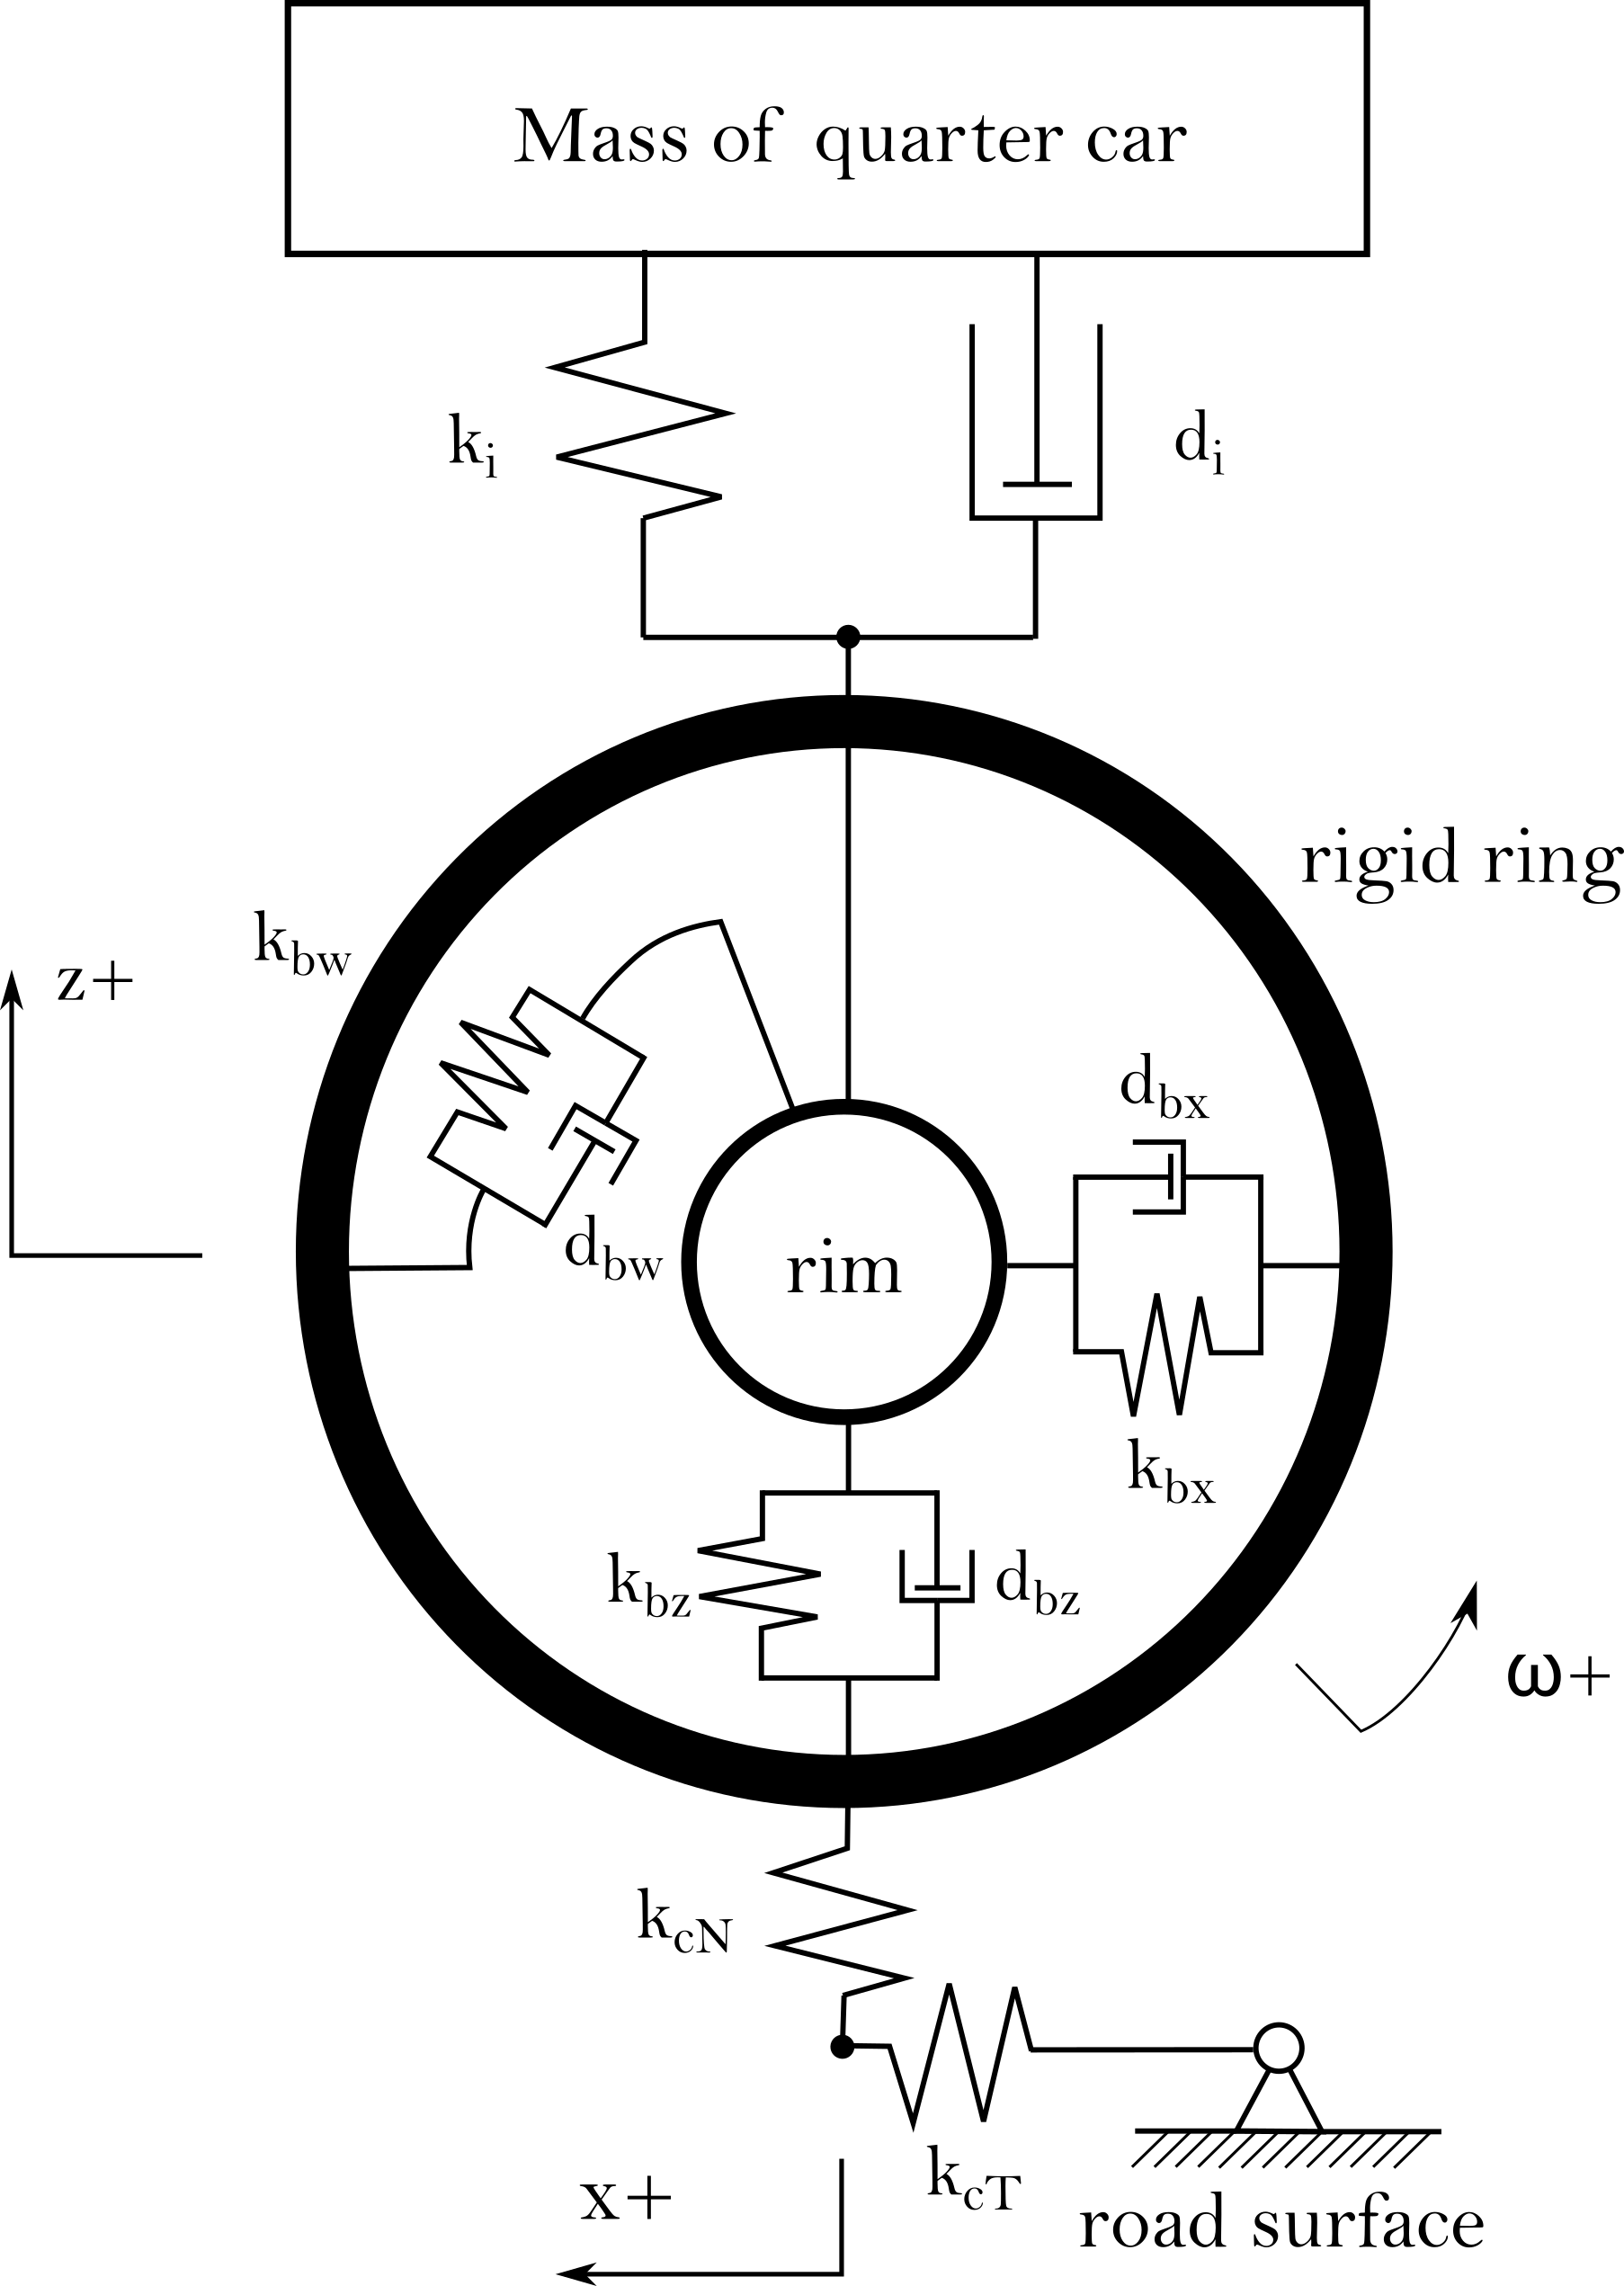
\includegraphics[width=0.4\textwidth]{bilder/rrm.png}
 \caption{Rigid ring model.}
 \label{fig:rrm}
 \end{figure}

The equations of motion for the rigid ring are

\begin{align}
\label{equ:rr}
m_b\ddot{x_b}+k_{bx}(x_b-x_r)+d_{bx}(\dot{x_b}-\dot{x_r}) &= cos\beta F_{cT}-sin\beta F_{cN} \\
m_b\ddot{z_b}+k_{bz}(z_b-z_r)+d_{bz}(\dot{z_b}-\dot{z_r}) &= -sin\beta F_{cT}-cos\beta F_{cN}\\
I_{by}\ddot{\omega_b}+k_{b\omega}(\omega_b-\omega_r)+d_{b\omega}(\dot{\omega_b}-\dot{\omega_r}) &=-r_eF_{ct}
\end{align}

where $k$ is the stiffness coefficient, $d$ is the damping coefficient, $F_{c}$ is the force from the contact patch, which $F_{cN}$ is the normal component and %F_{cT} is the tangential component.
%
$\omega$ is the effective road surface angle, and $r_e$ is the tire loaded radius.
%
The subscript 'r', 'b' and 'c' indicates the component rim, rigid ring and the contact patch).
%
The mass of the three components is denoted by $m$, the moment of inertia by $I_y$.

To implement the rigid ring tire model to the car model, we still need to build a force model for the $F_c$.
%
The normal force is the combination of the normal forces between the ground surface and the tread block due to the static quarter weight of the vehicle and the spring displacement and velocity damping between the ring and the tread block normal to the effective ground plane~\cite{na2016rigid}.
%
If the stiffness coefficient of the contact patch $k_cN$ and $k_cT$ are already known or can be measured.
%
The force $F_c$ is as

\begin{align}
\label{equ:contact_patch}
F_{cN} = k_{cN}(x_r-x_c)sin\beta+k_{cN}(z_r-z_c)cos\beta+Mg cos\beta \\
F_{cT} = k_{cT}(x_r-x_c)cos\beta+k_{cT}(z_r-z_c)sin\beta
\end{align}

If the stiffness coefficient of the contact patch is unknown or hard to measure.
%
\cite{zegelaar1998dynamic} introduces a way to describe the force of the contact patch, in which a residual deflection $\rho_{zr}$ is used to achieve a realistic overall tire stiffness.
%
The vertical force of the contact patch is resulted as

\begin{equation}
F_{cz} = q_{Fzr3}\rho_{zr}^3+q_{Fzr2}\rho^2+q_{Fzr1}\rho_{zr}+q_{V1}\Omega^2
\end{equation}

where $q$ indicate the coefficients set in~cite{} and $\Omega$ is the rim rotational velocity.
%
The residual deflection is as

\begin{equation}
\rho_{zr}=r-z_b+q_{V1}\Omega^2
\end{equation}

where $w$ is the effective road surface height.
%
The longitudinal force of the contace patch can be derived from the empirical Pacejka model.

\begin{equation}
F_{cx} = Asin(Barctan(Cs_x))
\end{equation}

where parameter $A,B,C$ have no direct physical meaing and are set from the system identification.
%
$s_l$ is the slip of the tire in the longitudinal direction and can be represented as

\begin{equation}
s_x=\frac{\dot{x_b}-r_e(\Omega+\dot{\theta_b})}{\dot{x_b}}
\end{equation}

Replacing the $m_ui$ as $m_r$ in the \ac{FCM} in Sec.~\ref{sec:active full car model}, then add the equation~\ref{equ:rr} of the rigid ring and the force model of the contact patch which is introduced in Equ.~\ref{equ:contact_patch} or in~cite{}, the rigid ring tire model is implemented in the \ac{FCM}.
%
It can be seen that in the rigid ring model the motion in the longitudinal direction is took into consideration, which is the advantage with the point contact tire model.
 
Besides, a more detailed and accuracy rigid ring model which is attended with a two or five point follower is introduced in \cite{na2016rigid}.
 
 
\subsection{Modified Point Contact Tire Model}
\label{sec:improved_pcm}
 
The rigid ring tire model is simple and efficient, but one additional consideration for developing the improved model is its suitability for using standard laboratory tests to measure the required lumped parameters for vertical, longitudinal, and torsional sidewall stiffness as well as tread, rigid ring, and bead/sidewall mass elements of four tires~\cite{na2016rigid}.

Cause the test laboratory is not available in the thesis, a modified point contact model is proposed to compromise the accuracy of the model and the financial situation.

The gain {$K$} is introduced to tune that is described as a function of the ratio {$e$} and the velocity of the vehicle {$v$}.


 \begin{equation}
 K=\begin{cases}
    a_0+a_1\cdot e^{a_2}\cdot v^{a_3} & (e < 1) \\
    1 & (e \geq 1)
 \end{cases}
 \end{equation}
 \label{form:K}
 
where

\begin{equation}
    e = \frac{l_{obstacle}}{l_{contact patch}}
\end{equation}

is the ratio between the length of obstacles and the tire contact patch.
%
$a_0, a_1, a_2, a_3$ are the factors of the description of the gain $K$.

When the tire crosses a obstacle, whose profile is below the road surface and its length is smaller than the tire contact patch, e.g a small and deep pothole or railway crossing, the height of the obstacle will be decreased in some degree by the gain.
%
The reason is that in this situation the real displacement of the wheel rim due to the elasticity of the rubber cannot be the same as the depth of the obstacles.

The situation is represented in Fig.~\ref{fig:tire}.
%
The real displacement of the wheel rim $\Delta z_u$ is smaller than the irregularity of the road profile $\Delta r$.
%
The less the ratio $e$ which represents a shorter obstacle wavelength, the slighter the influence from the obstacle on the displacement of the wheel rim.

 \begin{figure}
 \centering
 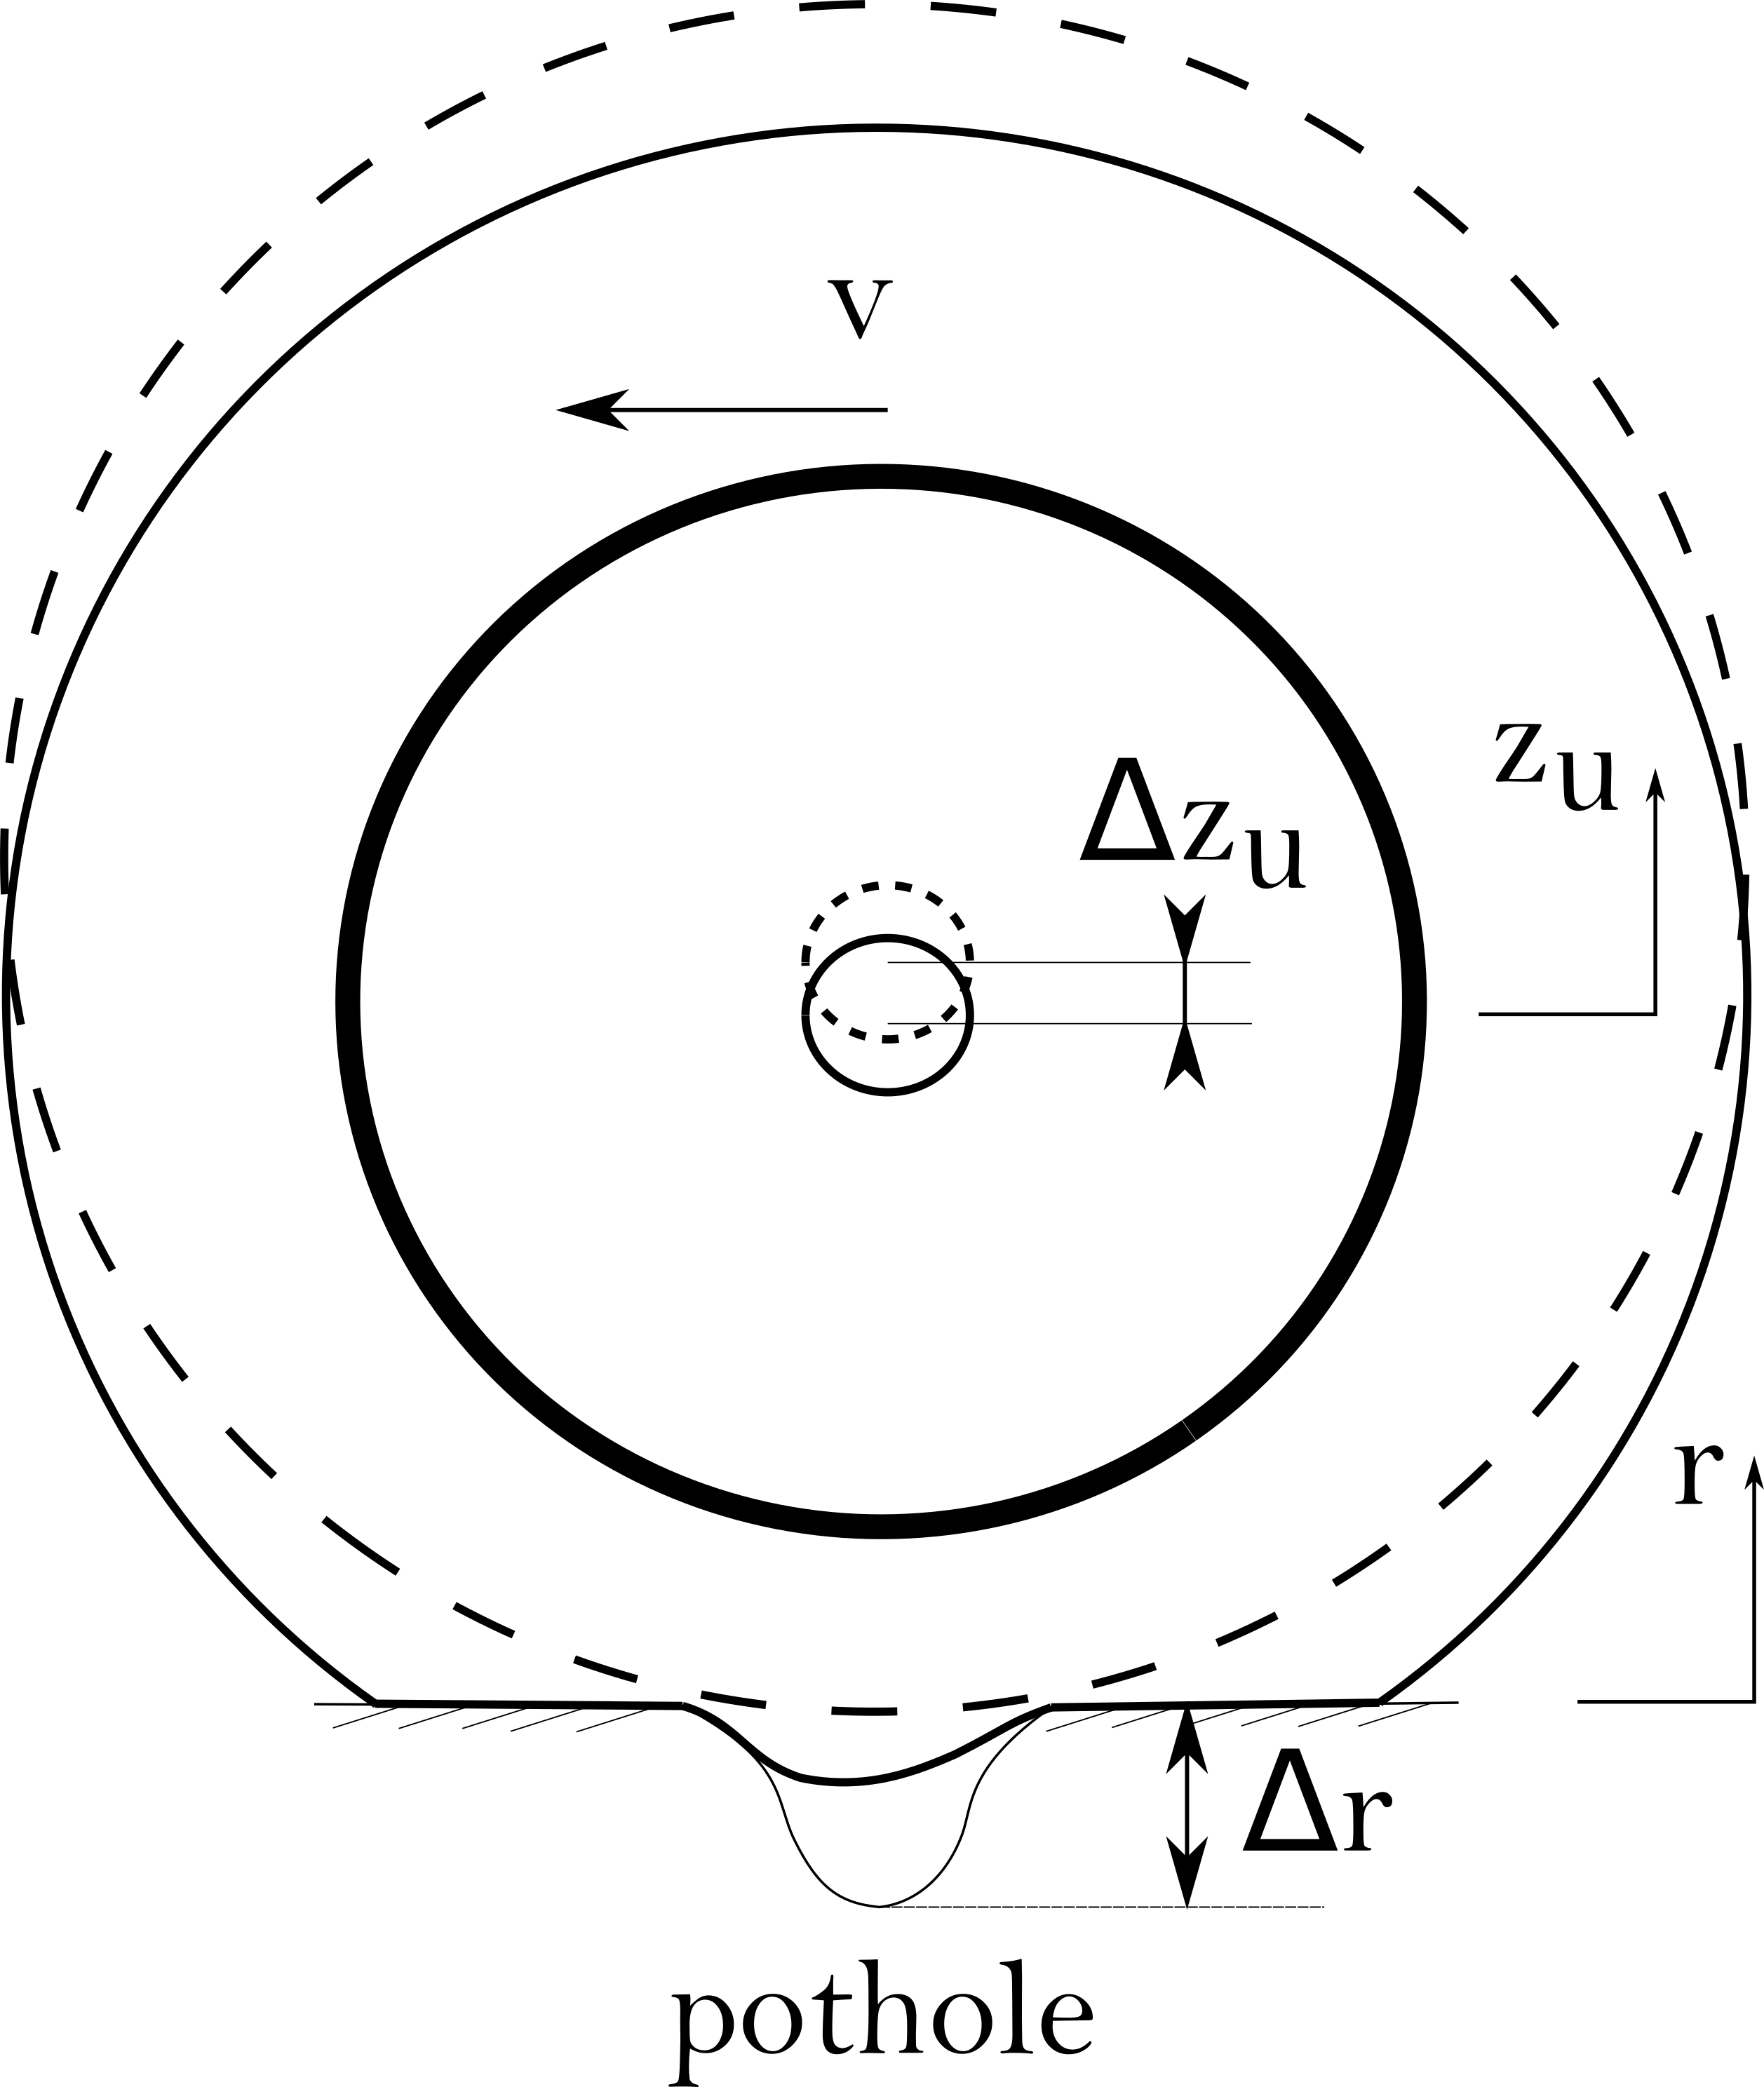
\includegraphics[width=0.3\textwidth]{bilder/tire.png}
 \caption{Contact situation with a short pothole.}
 \label{fig:tire}
 \end{figure}

While the tires crosses the obstacle whose profile is above the road surface and is steep, e.g a cleat or a step, the amplitude of the signal will be increased by $K$.
%
Except the vertical component of the velocity which will give an additional velocity to the wheel rim in vertical direction, the force that is generated during the crash by the obstacle has also a impact on the vehicle. 
%
The strength of the impact is related to the velocity of the vehicle.
%
The faster the velocity of the vehicle crosses the obstacle, the stronger the vibration is generated from the obstacle on the vehicle.

With this method the motion in the longitudinal direction and the interaction of the tire and the road have been considered in a simplified way.
%
The parameters {$a_0$}, {$a_1$}, {$a_2$}, {$a_3$} will be identified in Sections~\ref{sec:identification and validation}.